\chapter{Sensitivity of a flood-inundation model to rainfall distribution and erosional parameterisation}
\label{chapter_flood_model_sensitivity}
\chaptermark{Flood inundation model sensitivity}
%\begin{refsection}

%\begin{abstract}
%Landscapes evolve and take their shape from the cumulative effect of `geomorphically effective' events. In temperate climates, these are rainfall-driven events of sufficient magnitude to trigger threshold-dependent erosional processes. This chapter investigates the sensitivity of two end-member erosional models to the spatial resolution of rainfall input to a catchment using three historic severe rainfall events in Northern England and Cornwall.
%
%It is demonstrated that the erosional model chosen exerts first-order control of the total amount of landscape change and sediment flux. However, both end member models show sensitivity to the spatial resolution of rainfall input data during individual, formative rainfall events. 
%
%\end{abstract}
\section{Introduction}

%Flooding from intense rainfall poses great risk to communities living in proximity to rivers and has the potential to cause loss of life and substantial economic damage in affected areas \citep{pitt2008pitt}. Reliable prediction and advanced warning of flooding requires an understanding of the hydrological processes that operate within a river catchment, in order that flood forecasting models may be better parameterised and developed to mitigate against the impact of future events. Uncertainty in making hydrological predictions comes from a range of boundary conditions \citep{pappenberger2006influence} and many of these boundary conditions are known controls on catchment hydrology and causes of flooding \citep{shaw2010hydrology,sear2010guidebook}. Hydrological processes within the river catchment system are sensitive to a number of external and internal forcings, including but not limited to precipitation input \citep{nicotina2008impact}, catchment vegetation cover \citep{darby1999effect,andreassian2004waters,bradshaw2007global}, preconditioning of the catchment water table and soil moisture store by antecedent conditions \citep{berthet2009crucial}, urbanisation \citep{hollis1975effect}, debris mobilisation and blockage in river channels \citep{gippel1995environmental,jeffries2003influence}, as well as channel and floodplain morphological change during flood events \citep{werner2005spatially,wong2015sensitivity}. 


%Spatial resolution
The question of whether the hydrological response of a river catchment is sensitive to the spatial detail in rainfall input  is unresolved, with a number of different studies arriving at seemingly conflicting conclusions as to the exact role of rainfall spatial variability. One early study using deterministic modelling of river catchments and synthetic rainfall fields \citep{wilson1979influence} suggests that detailed space--time representations of rainfall are needed in distributed hydrological models to produce accurate flood forecasts. Predicting peak discharge in a small catchment (7.5km\(^2\)) is sensitive to the temporal resolution of rainfall input data, but less so to the spatial distribution of rainfall inputs during single storm events\citep{krajewski1991monte}. Over longer time scales (on the order of decades), a similar conclusion is reached by \citet{coulthard2016sensitivity}, finding that temporal resolution of rainfall input data is a greater control on hydrological outputs over long time periods than spatial resolution. 

The catchment size is likely to play a part in determining sensitivity to rainfall spatial distribution, with several studies suggesting smaller catchment sizes can dampen the effect of rainfall spatial variability \citep{segond2007simulation,nicotina2008impact}. The idea of catchment-size dependence has been developed further \citep{gabellani2007propagation}, to suggest that sensitivity to rainfall spatial heterogeneity depends on the characteristic size of the rainfall feature and the catchment size. Systematic investigation of the role of catchment size and morphology have suggested that the ratio between the characteristic hillslope length of the catchment and the rainfall feature determines sensitivity to rainfall spatial heterogeneity \citep{nicotina2008impact}. In cases where the rainfall feature is much greater in size than the typical hillslope length, the effects of rainfall spatial heterogeneity on runoff generation and hydrological response are limited. 

%Rainfall Radar
Modelling catchment hydrological sensitivity to rainfall spatial resolution requires a rainfall data source capable of capturing the spatial variability of rainfall across a catchment. Rainfall radar has been successfully used as a spatially variable rainfall input to a variety of types of catchment hydrology and urban hydrology models, from deterministic flood-inundation models \citep[e.g][]{coulthard2016sensitivity}, to probabilistic hydrology models \citep{bell2000sensitivity,cole2008hydrological}. The use of rainfall radar can be applied to modelling a range of environmental situations. For example, urbanised catchments \citep{berne2004temporal,einfalt2004towards,thorndahl2014analyses} to small mountain catchments \citep{borga2000use}, as well as large-scale regional hydrological modelling using national rainfall radar networks \citep{knebl2005regional}.

%Morphology change
Understanding how flood dynamics interact with channel and floodplain morphological change is of growing concern for flood modelling \citep{fewtrell2011geometric}. Morphological change during flood events has been shown to be a potential control on the extent of flooding during intense rainfall \citep{schumm1979geomorphic,stover2001channel,wong2015sensitivity}, particularly when river channels undergo geomorphically rapid change during repeated rainfall events of high magnitude \citep{sear2010guidebook,slater2016extent}. Within the context of a single flood, bedload sediment may become highly mobile, and the forces acting on the boundaries of the river channel are sufficient to alter channel geometry in long profile, cross-section, and channel pattern \citep{kleinhans2013splitting,wong2015sensitivity}. As a counterargument, during large flood events, the floodplain and river channel may effectively act as one channel unit, dampening any effects brought about by changes to river channel morphology \citep{bates2005numerical}. The implications of sediment transport and erosion within river catchments has been highlighted as an important factor in flood inundation modelling \citep{lane2007interactions,lane2008reconceptualising,neuhold2009incorporating}, and should form part of an effective flood modelling strategy \citep{wong2015sensitivity} in catchments thought to be sensitive to morphological change during large floods. Most numerical modelling approaches to flood inundation prediction are concerned with improving or addressing uncertainties in hydraulic flow \citep{galland1991telemac,bates2000simple}, rather than considering other boundary conditions such as the morphology of the channel bed and floodplain itself. Numerical models of flood inundation often overlook river channels and their floodplains as a mechanism for controlling flow patterns and inundation extents during flash floods \citep{neuhold2009incorporating}.

% Bring two together.
Flood inundation prediction studies rarely consider both geomorphological change or spatial heterogeneity in rainfall inputs to the catchment during intense rainfall episodes. Given the reported importance of rainfall resolution on predicting increased erosion rates, sediment yields and channel incision over decades \citep{deluis2010rainfall,coulthard2016sensitivity}, can the same observation be made at the time scale of a single event? In extreme rainfall events that mobilise large amounts of sediment, does this in turn control the dynamics and distribution of the floodwaters? Though there are different conclusions as to importance of rainfall heterogeneity and channel morphological change in flood inundation modelling, there is at least agreement that both have the potential to alter the outcome of flood prediction under certain conditions -- yet exactly which conditions is still uncertain. More investigation is needed into which of these uncertainties -- spatial heterogeneity of rainfall input or erosional processes -- plays the greater role in determining flood inundation patterns during intense rainfall events. The simulations and analysis presented in this chapter attempts to address this by comparing flood inundation model predictions under different rainfall spatial resolution scenarios and erosion law parameterisations. 

%Climate impact etc.
%Growing consensus indicates that intense rainfall events are becoming more frequent in the UK \citep{kendon2014heavier}.

The following questions are explored through the use of numerical modelling experiments set out in Chapter \ref{chapter_events}.

\begin{enumerate}
\item Are predicted flood inundation extents during a storm sensitive to the spatial resolution of rainfall inputs to the catchment?
\item Is morphological change of the floodplain and channel during a storm event substantial enough to affect flood inundation predictions?
\end{enumerate}

\section{Method}

An ensemble of numerical simulations detailed in Chapter \ref{chapter_events} is used to investigate catchment hydrological response to different parameterisations of spatial variability of rainfall data and erosional process representation. The ensemble simulations use the HAIL-CAESAR landscape evolution model developed in Chapter \ref{chapter_HAIL-CAESAR}. The results of the simulations were then analysed in terms of the hydrological outputs of the model: water discharge, average water depths, and spatial distribution of floodwaters. The set of simulations used in this chapter are laid out in Table \ref{table_ensemble_experiments} in Chapter \ref{chapter_events}. In addition to the simulations described in Chapter \ref{chapter_events}, a further set of hydrological simulations is carried out to assess the model sensitivity to the \(m\) hydrological parameter that controls how rapidly the catchment responds to rainfall events \citep{beven1979physically}.

\subsection{Sensitivity analysis of the TOPMODEL \(m\) parameter}
There are numerous user-defined parameters in the HAIL-CAESAR model (and in landscape evolution models in general) that have a wide range of potential values. Parameter selection in environmental modelling comes with a degree of uncertainty, and resulting outputs from models can be highly sensitive to the user's choice of input parameters for a given simulation \citep{Pelletier2012}. Initial testing of the HAIL-CAESAR model, and studies using the CAESAR-Lisflood model that it is based upon, show it is particularly sensitive to the \textit{m} parameter \citep{coulthard2002cellular,welsh2009testing}. The \(m\) parameter in HAIL-CAESAR is based upon an adaptation of the semi-distributed hydrological model TOPMODEL \citep{beven1979physically}. The parameter represents the rate of the rise and fall of the soil moisture store, determining how quickly a catchment responds to rainfall inputs -- sometimes referred to as the `flashiness' of a catchment. A high value of \(m\) reduces the transmissivity of the soil, leading to slower response times in the catchment, whereas a lower value of \(m\) increases soil transmissivity leading to quicker response times to rainfall input and a `flashier' hydrograph. The \(m\) value imitates the factors associated with water movement and storage in relation to the vegetation cover of a catchment; it is sometimes termed the \textit{land-use parameter} \citep{welsh2009testing} to reflect this. Typical values used for \(m\) range from 0.002--0.005 (grassland) to around 0.02 (dense forest) with the range of values in between representing a full range of vegetation covers \citep{beven1984testing,beven1997topmodel}.

Initially, the experiments were designed to use the default model value of \(m = 0.002\) for grassland -- both the Boscastle and Ryedale catchments are a mixture of agricultural pasture land, some sparse vegetation, and small urban settlements -- but the dominant land cover is sparse vegetation. The default value for \(m\) was adequate in reproducing the Boscastle hydrograph noted in an earlier study \citep{wallingford2005flooding}, but the hydrological response of the Ryedale catchment was highly sensitive to the choice of \(m\) parameter. To assess the full range of sensitivity to the choice of \textit{m} parameter in the Ryedale catchment, a series of simulations were carried out with a range of \textit{m} values for both uniform and gridded rainfall inputs. Simulations of each flood event were carried out with the \textit{m} values shown in Table \ref{table-m-sens}. Each of the simulations was run with the model in hydrology-only mode, with no erosional process parameterisation switched on. To assess whether there was further sensitivity to the type of rainfall input (gridded or uniform), the sensitivity analyses were repeated with both types of rainfall input data.

\begin{table}
\begin{tabular}{lc}
\textbf{Catchment} & \textbf{\(m\) parameter} \\
\hline
%Boscastle   &                                            \\
Ryedale     & 0.003, 0.004, 0.005, 0.006, 0.007, 0.008, 0.009, 0.01, 0.015, 0.02  \\
\hline
\\ 
\end{tabular}
\caption{TOPMODEL \(m\) parameter values used to run sensitivity simulations for each type of rainfall input types (Uniform and Gridded) for the Ryedale catchment. }
\label{table-m-sens}
\end{table}

%%%%%%%%%%%%%%%%%
\section{Results}
%%%%%%%%%%%%%%%%%

\subsection{Model sensitivity to the \(m\) parameter}

The model exhibited a strong sensitivity to the choice of the TOPMODEL \(m\) parameter. In the results presented in Figure \ref{fig_topmodel_m_ryedale_lumped} peak river discharge ranged from approximately 530 m\(^3\)s\(^{-1}\) using an \(m\) value of 0.003 to 20 m\(^3\)s\(^{-1}\) using an \(m\) value of 0.008 under uniform rainfall input conditions. Under spatially variable rainfall inputs, discharge was as high as 650 m\(^3\)s\(^{-1}\) where \(m = 0.003\). The measured peak discharge reported for the 2005 Ryedale storm at the Ness gauging station was 80 m\(^3\)s\(^{-1}\) (Environment Agency, email communication), and a subsequent post event report estimated the peak discharge at 105 m\(^3\)s\(^{-1}\) \citep{wass2008investigation}. In the sensitivity simulations, a value of \(m = 0.005\) under uniform rainfall conditions produced a flood peak most closely matching the observed value, peaking at approximately 100 m\(^3\)s\(^{-1}\), the choice of \(m=0.005\) for Ryedale also best approximated the timing in the rise and fall of the hydrograph. Under spatially variable conditions (Figure \ref{fig_topmodel_m_ryedale_gridded}), a value of \(0.007 < m < 0.008\) would appear to produce a hydrograph most likely to match the observed discharge rates in terms of the onset of flooding, but a value of \(0.006 < m < 0.007\) would be likely to more closely match the magnitude of peak discharge. At a first approximation, the use of uniform rainfall inputs appeared to lead to better agreement of the model with measured discharges from the river gauging station data, in terms of agreement with both the timing and magnitude of the flood peak. It was decided therefore to use the calibration data from the uniform rainfall sensitivity analysis to choose the best value of \(m\) for the main set of simulations. 

There were differences between the hydrographs of the observed and simulated discharges in terms of peak discharge timing and recession limb shape. The measured hydrograph overlaid in Figure \ref{fig_topmodel_m_ryedale_lumped} (black dashed line) showed a sharp rise at around 50 hours after the start of the simulation period. Lower \(m\) values (\(m < 0.005\)) resulted in the prediction of the flood peak being too early compared to the observed timing, with values \textgreater \ 0.005 predicting the flood peak timing too late. Most of the simulations failed to capture the extended duration of peak discharge, which lead to a `plateaued' appearance of the measured hydrograph, lasting approximately 5--6 hours, before receding back to low flow levels. The simulation with \(m = 0.006\) came closest to predicting this plateaued hydrograph shape, but failed to predict the magnitude of water discharge correctly, underestimating the peak flow by almost 50\%. 

For Ryedale simulations, it was decided to use an \(m\) value of 0.005, providing the closest possible match to the flood peak discharge, though not the true shape of the hydrograph and the receding limb. As the catchment simulations include a representation of erosion and sediment transport processes, which are often threshold dependent, it was felt necessary to match the discharge peak more closely over choosing to match the hydrograph shape precisely.

% comment on second run with gridded rainfall in ryedale

\begin{figure}[!h]
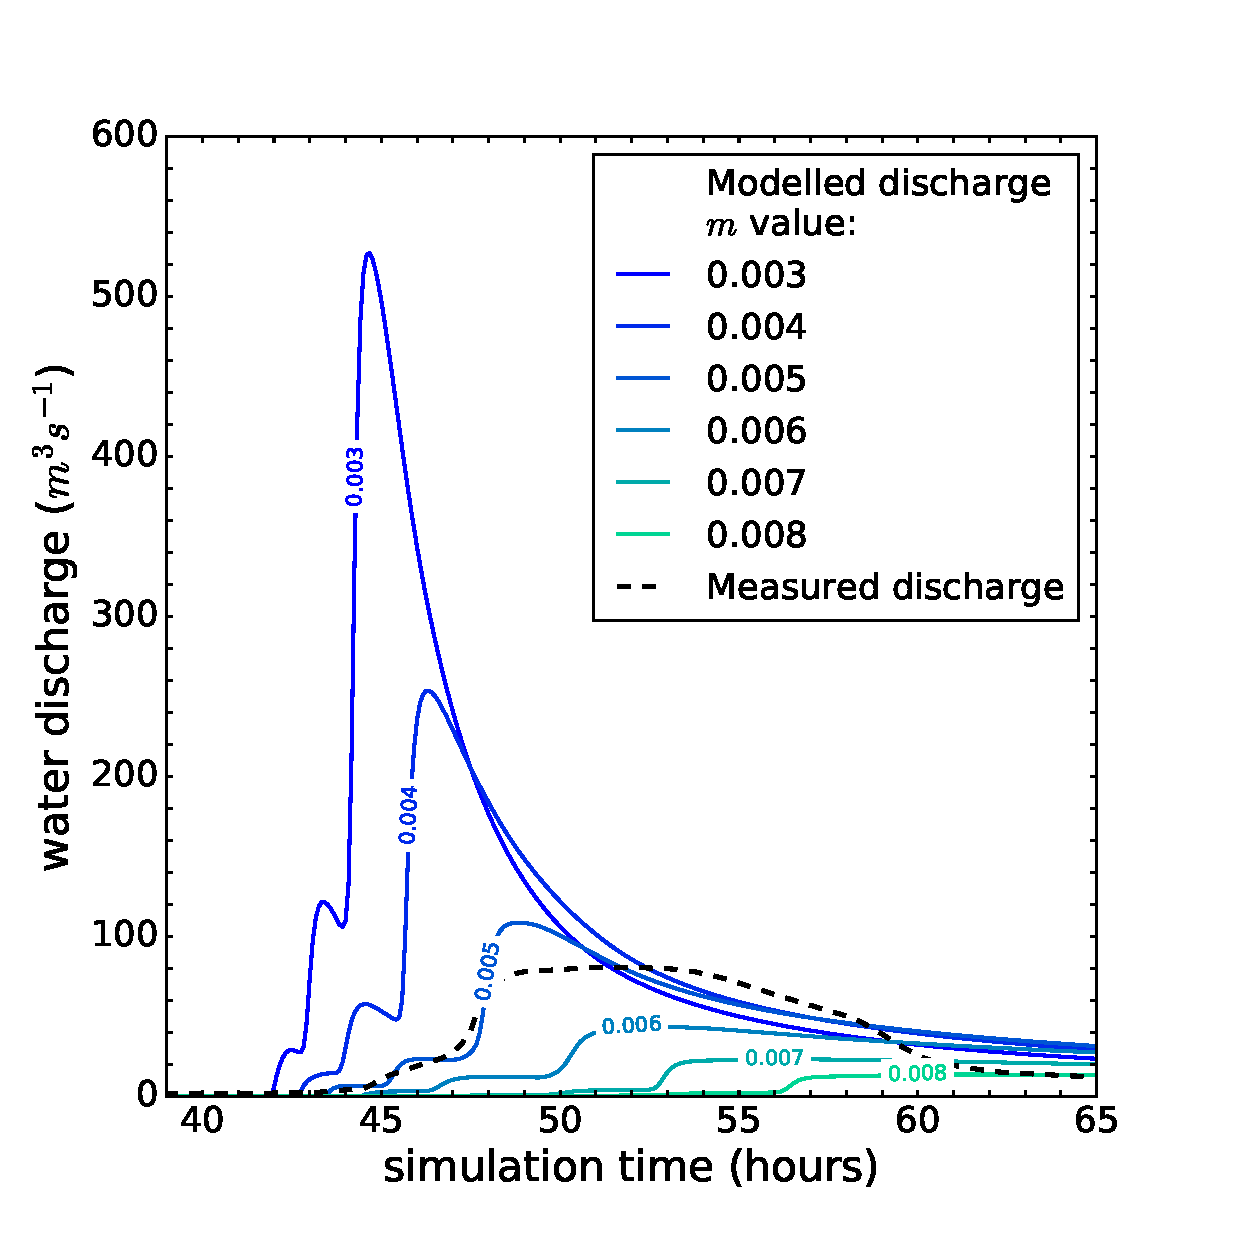
\includegraphics[width=11cm]{chp_flood_figs_scripts/fig_ryedale_hydro_m_sens_lumped.eps}
\caption{Hydrograph sensitivity to the \(m\) parameter under \textbf{uniform} rainfall inputs. Discharge over time at the Ryedale catchment outlet for varying values of the \(m\) parameter. The measured discharge at the catchment gauging station is overlaid in dashed line. The results from the simulations with \(m\) \textgreater \ 0.008 are omitted for clarity due to the low discharges they produced.}
\label{fig_topmodel_m_ryedale_lumped}
\end{figure}

\begin{figure}[!h]
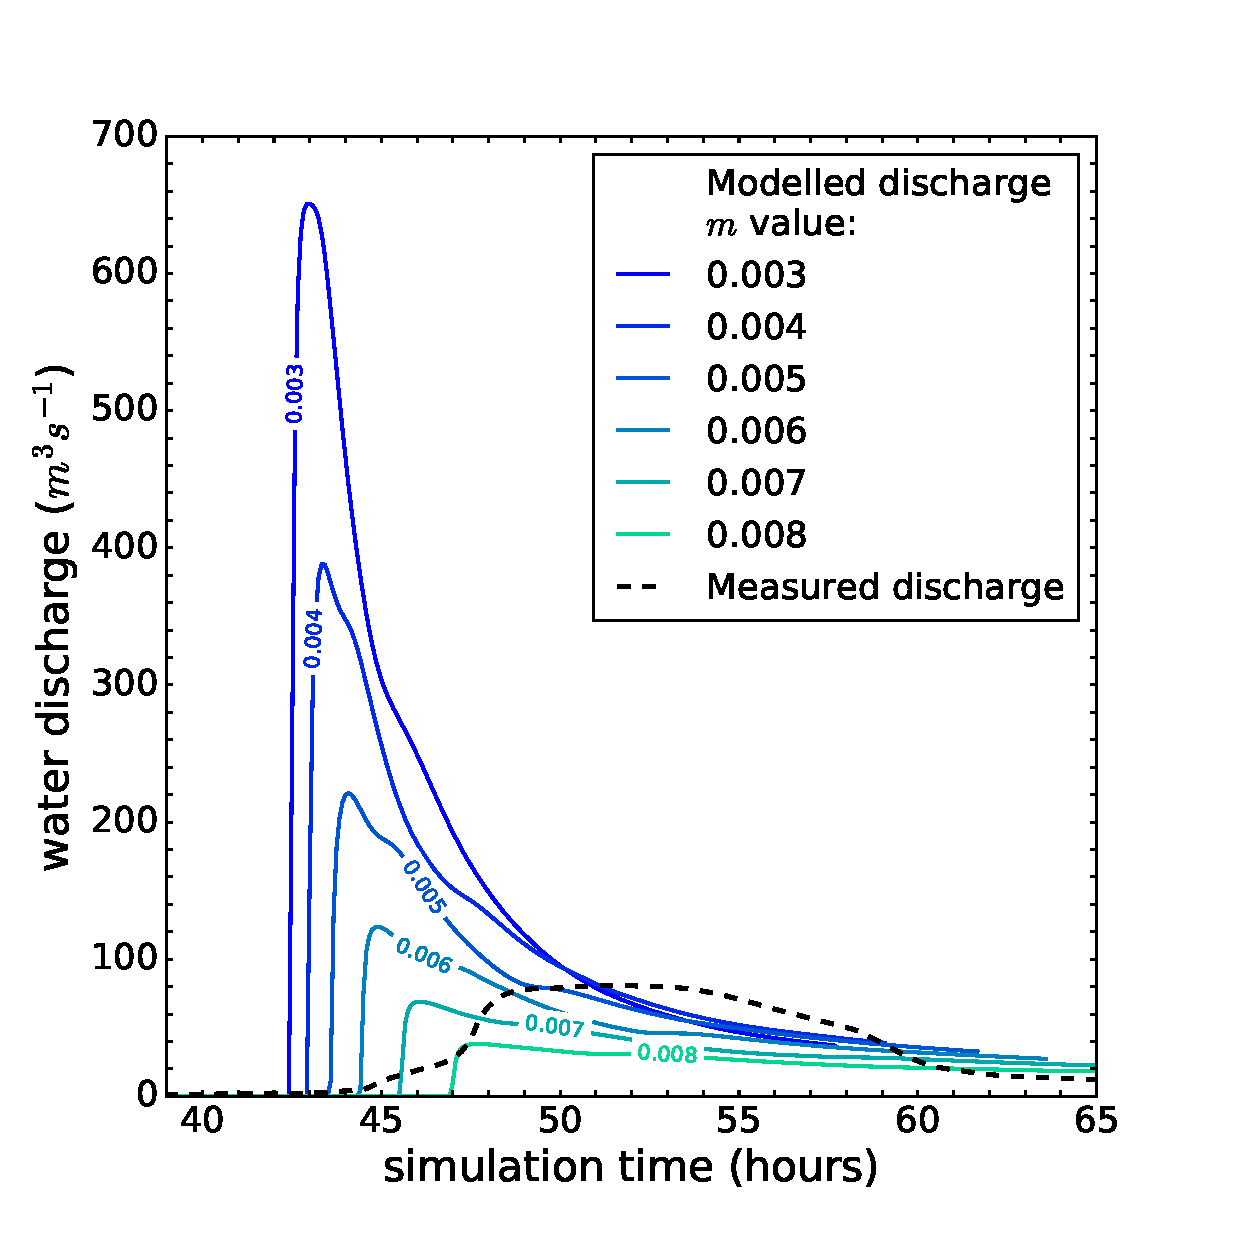
\includegraphics[width=11cm]{chp_flood_figs_scripts/fig_ryedale_hydro_m_sens_gridded.eps}
\caption{Hydrograph sensitivity to the \(m\) parameter under \textbf{gridded} rainfall inputs. Discharge over simulation time at the Ryedale catchment outlet for varying values of the \(m\) parameter. The measured discharge at the catchment gauging station is overlaid in dashed line. The results from the simulations with \(m\) \textgreater \ 0.008 are omitted for clarity due to the low discharges they produced.}
\label{fig_topmodel_m_ryedale_gridded}
\end{figure}

\subsection{Catchment hydrographs}
\label{sec_hydrographs_flood}
% AMMENDMENTS:
%Plot hyetograph (rainfall) oerlay on the hydrographs.
%For Ryedale, plot the measured observation as well from gauge. -done

%Comparisons with the actual hydrographs from the gauged basins?
\subsubsection{General observations}
At the catchment scale, hydrological response was sensitive to both the rainfall resolution and the choice of erosional model. For both catchments, higher resolution rainfall input data resulted in a greater maximum river discharge. In the Ryedale experiments, simulations using the gridded rainfall input experienced a flashier hydrological response, reaching peak discharge several hours before the uniform rainfall input cases. This large difference in timing was not observed in any of the Boscastle simulations, with all simulations reaching peak discharge within 10 minutes of each other. Peak discharges and the timings of peak flow for each simulation are tabulated in Table \ref{table_discharges}.

The choice of erosion model also influenced the hydrological response. When catchment erosion was modelled using a transport-limited (\texttt{TLIM}) case, peak discharges were higher in all cases, but the timing of hydrograph peaks remained similar for each case. The difference in peak discharges was minimal when comparing the detachment-limited (\texttt{DLIM}) cases to the hydrology-only simulations.

\subsubsection{Boscastle}
The timing of peak discharge in the Boscastle catchment was similar for both the gridded and uniform rainfall simulations (Figure \ref{fig_boscastle_hydrograph_ensemble}). In gridded rainfall simulations the discharge peaked 40 hours after the start of the simulation (1600 UTC) and for the uniform rainfall input simulations at 40 hours 10 minutes into the simulation (1610 UTC). The choice of erosional parameterisation did not appear to affect the timing of the peak discharge. However, it did result in small changes in the discharge rate at peak flow, of up to 14\% difference in the uniform rainfall simulations, and 6\% increase in the gridded rainfall simulations. The primary control on the amount of discharge at peak flow appeared to be the type of rainfall inputs into the model, with the gridded simulations predicting peak discharges up to 28\% higher than their uniform counterparts. 

Comparison with measured discharge is not possible in the Boscastle case, as the basin is ungauged. However, a number of methods exist for predicting runoff and river flow in ungauged river basins \citep{sivapalan2003prediction,bloschl2013runoff}, and two estimations of discharge are presented here for comparison with the predictions from the HAIL-CAESAR model. Both estimations were derived in the \citet{wallingford2005flooding} report and the hydrographs are overlaid on the model outputs from this study in Figure \ref{fig_boscastle_hydrograph_ensemble}. The HR Wallingford report produced a simple hydrograph derived from eyewitness reports and water level marks, estimating a peak discharge of 180 m\(^3\)s\(^{-1}\) at 1600 UTC, the same as the timing of peak flow in the HAIL-CAESAR simulations. A second estimation of the hydrograph during the Boscastle event was made in the report using a one-dimensional hydraulic model, InfoWorks RS, which also predicted a peak flow of approximately 178 m\(^3\)s\(^{-1}\), but at the later time of 1700 UTC. The InfoWorks RS model uses a fixed representation of the river bed; in other words, it does not permit the topographic surface to change during the course of the model simulation. 

The estimated flow from observations and the 1D hydraulic model was higher than any of the model predictions made in this study -- a difference of 30--80 m\(^3\)s\(^{-1}\) was noted between the HAIL-CAESAR simulations and the two estimations from the HR Wallingford report. The rising and falling limbs of the hydrograph were also much shallower than the HAIL-CAESAR model predictions, which suggest a much more rapid rise and fall in water levels during the storm. 

\subsubsection{Ryedale}

The hydrological response of the Ryedale catchment was more sensitive to the choice of rainfall input type, with marked differences in the timing and magnitude of the peak discharge between the uniform and gridded rainfall sets of simulations (Table \ref{table_discharges}, Figure \ref{fig_ryedale_hydrograph_ensemble}). There is up to 83\% increase in discharge in the gridded rainfall simulations when compared to the corresponding uniform rainfall input simulations. The hydrograph was less sensitive to the type of erosional parameterisation, with up to 40\% difference observed in the uniform rainfall cases, and upto 25\% difference in the gridded rainfall simulations. 

The River Rye is gauged at several locations, and flow data was recorded during the 2005 flood, though the accuracy of gauging station data is uncertain during particularly high flow events \citep{shaw2010hydrology}. The gauge data is measured at the River Rye Ness gauging station\footnote{Environment Agency gauging station F2505 -- British National Grid reference SE 69439 79196}. The outlet of the modelled catchment domain was set up to coincide (as near as possible) with the location of the Ness gauging station on the River Rye. The observed flow data from the gauging station is overlaid in Figure \ref{fig_ryedale_hydrograph_ensemble}. The gauging station data most closely matches the hydrographs produced by the uniform rainfall inputs, though it is lower than all of the simulated hydrograph, peaking at approximately 81 m\(^3\)s\(^{-1}\). A further value of peak discharge during the Ryedale flood was reported by \citet{wass2008investigation} as 105 m \(^3\)s\(^{-1}\), derived from 1D flow modelling -- the timing of this estimated peak flow was not available due to the type of model used. The value of peak discharge reported by \citet{wass2008investigation} is similar to that of the Environment Agency gauge data and the peak flows predicted by the uniform rainfall input simulations in this study. 

The difference in timing of peak flow between the set of gridded rainfall input simulations and the uniform rainfall simulations is large; the gridded rainfall simulations predict the timing of peak flow being almost four hours earlier than the simulations using a uniform rainfall input. Observations reported in \citet{wass2008investigation} and the Environment Agency gauge support the predictions made by the uniform rainfall simulations in this case.

% Please add the following required packages to your document preamble:
% \usepackage{graphicx}
\begin{table}[!htbp]
\centering
\caption{Peak water discharges and corresponding times at peak flow for each of the simulation cases. Discharge is calculated at the outlet of the catchment model domain. Time is given in UTC on the day of the storm.}
\label{table_discharges}

\begin{tabular}{lcc}
\textbf{Simulation name} & \begin{tabular}[c]{@{}l@{}}\textbf{Peak discharge}\\ (m$^3$s$^{-1}$)\end{tabular} & \begin{tabular}[c]{@{}l@{}}\textbf{Time}\\ (UTC on storm day)\end{tabular} \\
\hline 
\multicolumn{3}{l}{Boscastle: 2004-08-16} \\
\hline
\texttt{GRIDDED\_HYDRO} & 151 & 1600 \\
\texttt{GRIDDED\_TLIM} & 148 & 1600 \\
\texttt{GRIDDED\_DLIM} & 143 & 1600 \\
\texttt{UNIFORM\_HYDRO} & 108 & 1610 \\
\texttt{UNIFORM\_TLIM} & 122 & 1610 \\
\texttt{UNIFORM\_DLIM} & 107 & 1610 \\
\hline
\multicolumn{3}{l}{Ryedale: 2005-06-19} \\
\hline
\texttt{GRIDDED\_HYDRO} & 221 & 2005 \\
\texttt{GRIDDED\_TLIM} & 277 & 1950 \\
\texttt{GRIDDED\_DLIM} & 232 & 2000 \\
\texttt{UNIFORM\_HYDRO} & 108 & 0050$^\dagger$ \\
\texttt{UNIFORM\_TLIM} & 151 & 2340 \\
\texttt{UNIFORM\_DLIM} & 114 & 0025$^\dagger$\\
\hline
\vspace{1em}
{\footnotesize $\dagger$ -- Time the following day}. & & \\

\end{tabular}%
\end{table}

% ENSEMBLE HYDROGRAPHS
\begin{figure}[!htbp]
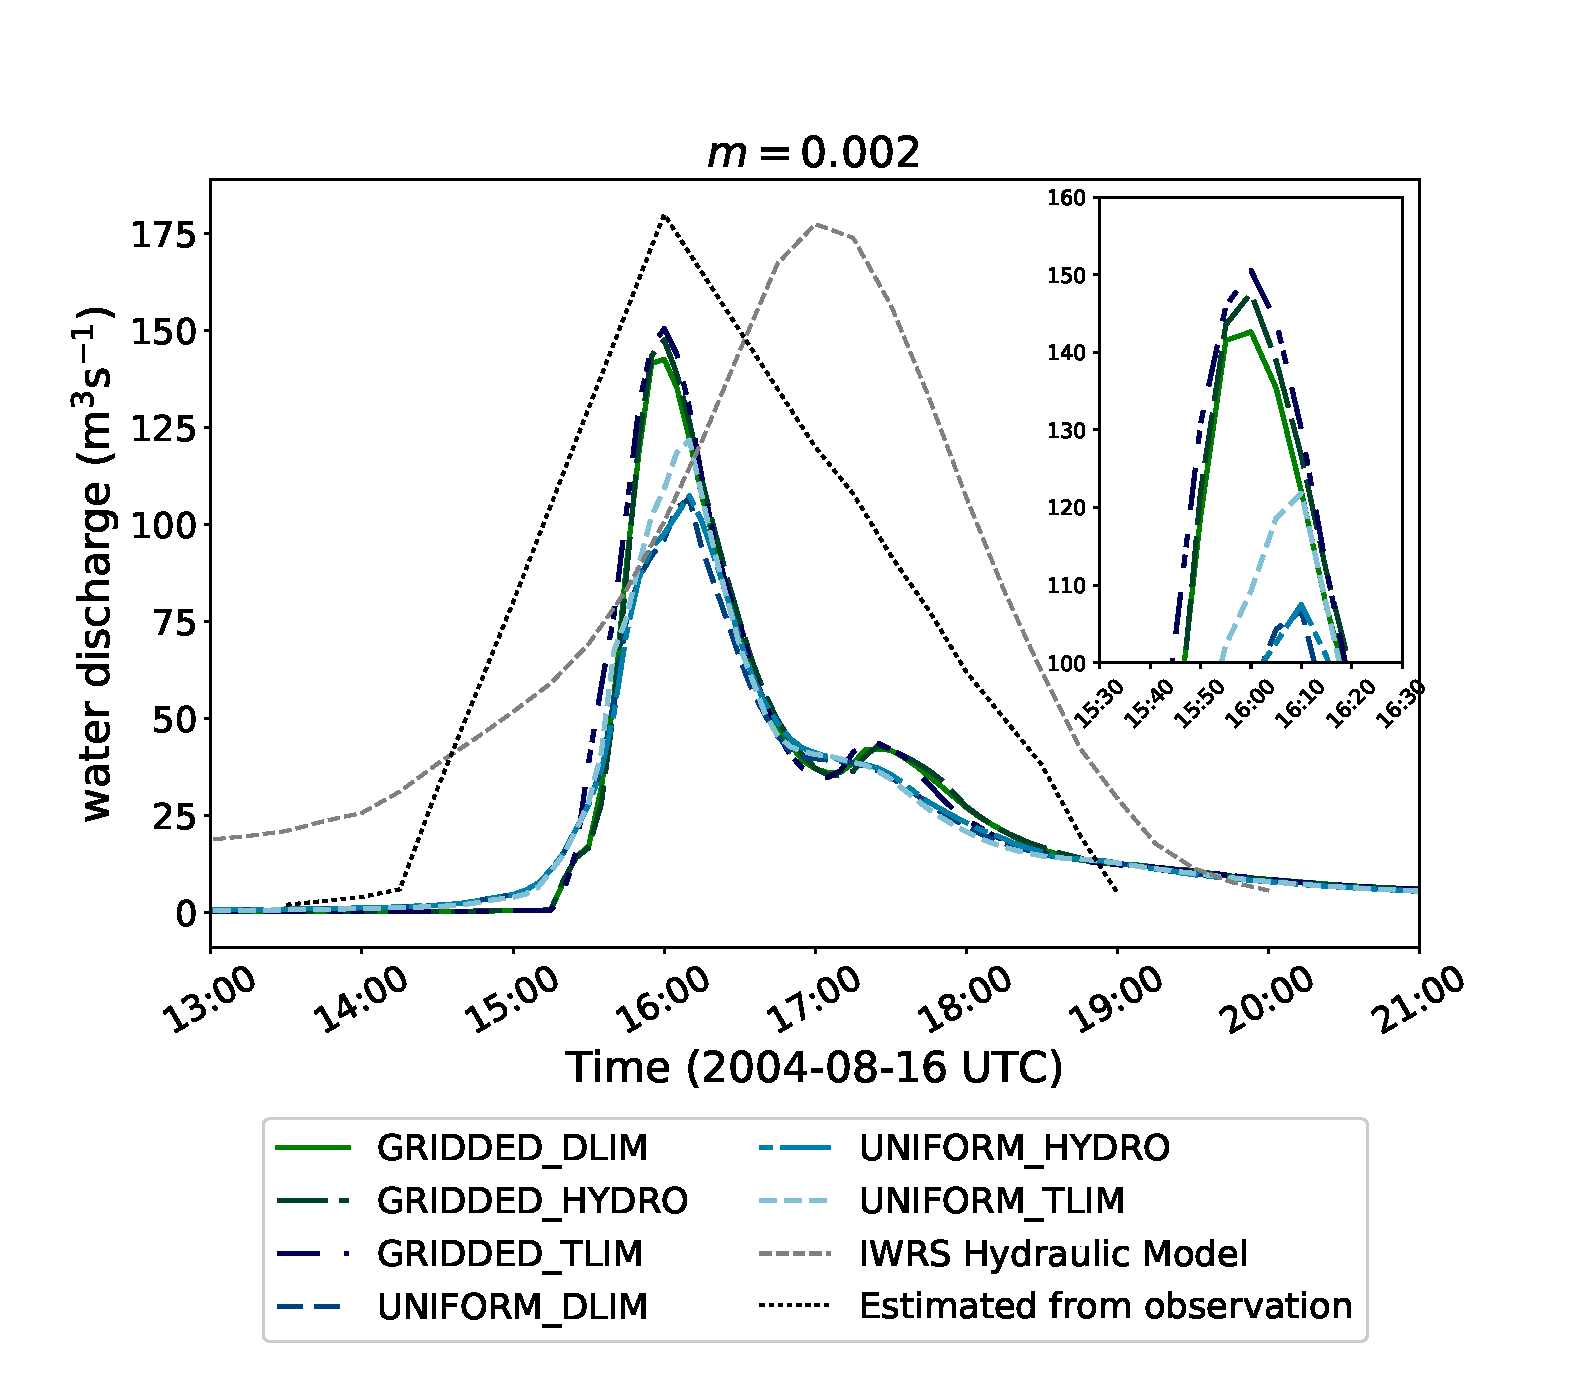
\includegraphics[width=14cm]{chp_flood_figs_scripts/fig_hydrographs_boscastle_new.eps}
\caption{Boscastle hydrographs (discharge over time at catchment outlet) for each simulation of the 2004 Boscastle event listed in Table \ref{table_ensemble_experiments}. Inset shows detail of main flood peaks around hour 40 of the simulation.}
\label{fig_boscastle_hydrograph_ensemble}
\end{figure}

\begin{figure}[!htbp]
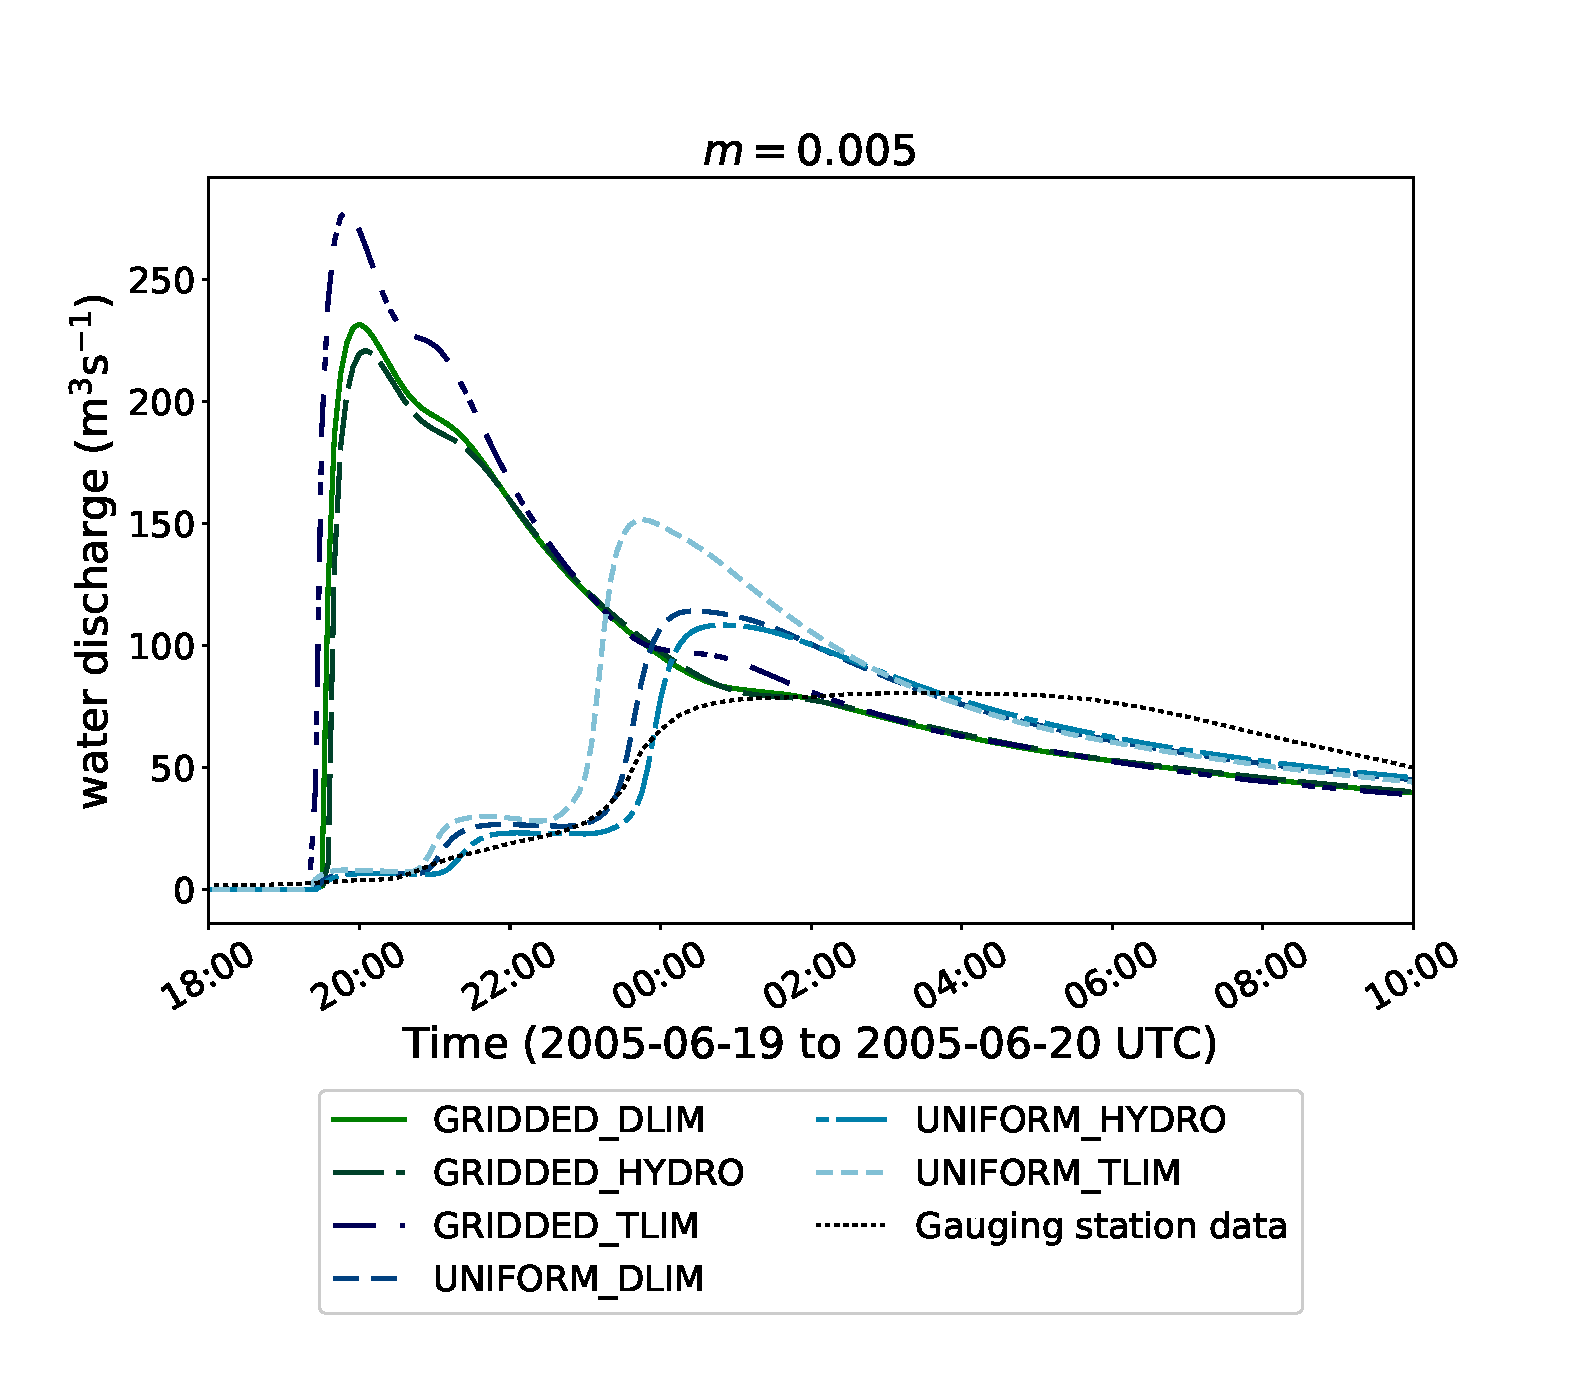
\includegraphics[width=14cm]{chp_flood_figs_scripts/fig_hydrographs_ryedale_new.eps}
\caption{Ryedale hydrographs (discharge over time at catchment outlet) for each simulation of the 2005 Ryedale event listed in Table \ref{table_ensemble_experiments}.}
\label{fig_ryedale_hydrograph_ensemble}
\end{figure}

\subsection{Flood inundation and river levels}
A series of flood inundation metrics are shown in Figures \ref{fig_inundation_area_ensemble}, \ref{fig_floodplain_depth_ensemble}, and \ref{fig_channel_depth_ensemble}, showing respectively:

\begin{enumerate}
\item Total area inundated by water
\item Mean water depth in the floodplain
\item Mean water depth in the main channel
\end{enumerate}

The floodplain area is defined for the purpose of this analysis using the \citet{clubbinpress} floodplain delineation algorithm, a method which searches for statistically significant variation in terrain relief to identify and delineate floodplains in a catchment. The `main channel' is herein defined as the mainstem channel with the highest stream order number \citep{strahler1957quantitative}, removing any tributary channels in the headwaters. The mainstem channel is delineated using a simple channel network identification algorithm based on a contributing drainage area threshold \citep{ocallaghan1984extraction,tarboton1991extraction}. The inundation metrics were derived from water depth output files created every two hours of simulated time during the model runs. As such, the absolute peak flood inundation may lie between two of the output file timesteps, but sufficient detail in spatial extents and dynamics of  the floodwaters are still captured in the analysis and the resulting figures. 

Generally, there is a tendency for the simulations with gridded rainfall input  running in hydrology-only mode (\texttt{GRIDDED\_HYDRO}) to predict the greatest extents of areal flood extent as well as floodwater depth across the floodplain and main river channel, behaviour observed in both case studies. Most simulations running in hydrology-only mode and uniform rainfall input (\texttt{UNIFORM\_HYDRO}) also predict greater flood inundation extents and peak water levels, but this tendency is less prevalent in the Ryedale simulations. In fact, the Ryedale simulations appear to be marginally more sensitive to the type of rainfall input, with both the \texttt{GRIDDED} simulations producing slightly higher peak inundation levels, regardless of whether erosion parameterisation is switched on in the model.

The starkest contrast observed was in the mean channel water depth of the Boscastle set of simulations; the difference in peak mean water depth was approximately 1 m between the hydrology-only and erosion-enabled simulations. In most of the other simulations, the differences in main channel mean water depth were smaller, on the order of tens of centimetres.

\subsubsection{Total inundation area}
Inundation area is defined here as the total area of the catchment grid cells that exceed the minimum discharge threshold at a given timestep. The minimum discharge threshold for all simulations was set as 0.03 m\(^3\)s\(^{-1}\). The inundation amounts for the Boscastle and Ryedale simulations are presented in Figure \ref{fig_inundation_area_ensemble}. For clarity, only results from one type of the erosion-enabled simulations is presented in each case (transport-limited -- \texttt{TLIM}). The predicted inundation areas for the detachment-limited erosion simulations were similar to the hydrology-only simulations, differing only by a few percentage points.

\paragraph{Boscastle}
Both of the hydrology-only simulations in the Boscastle case predicted the greatest peak in flood inundation area, with the gridded rainfall input simulations predicting slightly higher peak inundation areas. The highest predicted flood inundation area resulted from the \texttt{GRIDDED\_HYDRO} simulation, and the lowest peak from the \texttt{UNIFORM\_TLIM} simulation. The rise and fall in the areal extent of the inundated flood area is rapid, peaking within hour 40 of the simulation  (1600 UTC) and reducing by approximately 50\% by the next output time step, two hours later at 1800 UTC. 

\paragraph{Ryedale}
In the Ryedale simulations, predicted flood inundation area was again greatest in the \texttt{GRIDDED\_HYDRO} simulation and lowest in the \texttt{UNIFORM\_TLIM} simulation. In this set of simulations, both the gridded rainfall input experiments produce higher total inundation areas at the peak of the flood.

\subsubsection{Floodplain mean water depth}

Inundation area provides a general indication of the spatial extent of flooding within a catchment, but does not reveal as much about the distribution of water depths within the catchment, particularly the floodplain where many settlements are located in the Boscastle and Ryedale cases. Average floodplain water depths area presented in Figure \ref{fig_floodplain_depth_ensemble} showing how water depths rise and fall on the floodplain over the course of each storm. The average depth is calculated for each output time step (two-hourly), by averaging the water depth in each model grid cell, limited to area delineated by the floodplain-finding algorithm \citep{clubbinpress}. 

\paragraph{Boscastle}
Floodplain average water depths follow a similar pattern to that observed in the total inundation area timeseries: a sharp rise and peak corresponding to the time of maximum river discharge (1600 UTC), followed by a rapid drop-off by the time of the next model output timestep at 1800 UTC. Average water depths in the Boscastle floodplain peaked at just over 0.4 m for the \texttt{GRIDDED\_HYDRO} simulations. Average floodplain water depths for the other simulations were approximately 0.35 m, and showed little variation from this value between the different simulation parameters. %Overall there was little difference in average floodplain water depth (5 cm) predicted for the Boscastle event. 

\paragraph{Ryedale}
Water depths on the Ryedale floodplain were fast to reach their peak, but showed a more gradual recession after the flood peak than the Boscastle simulations. The highest mean floodplain water depths were predicted by the \texttt{GRIDDED\_HYDRO} simulations at 0.16 m, though the difference between other simulations was minimal -- the lowest predicted mean depths of 0.14 m were observed in the \texttt{UNIFORM\_TLIM} simulation, a difference of only 2 cm. The timings of peak water depth were slightly different between the gridded rainfall and uniform rainfall simulations, with uniform rainfall input simulations peaking 2--3 hours after the gridded rainfall input simulations, mirroring the pattern seen the Ryedale hydrographs (Figure \ref{fig_ryedale_hydrograph_ensemble}).

\subsubsection{River channel water depth}
Water depths in the river channel are determined by reporting the water depth along the channel midpoint, determined by a channel network extraction algorithm \citep{Braun2013}. Modification of the floodplain finding algorithm was considered to extract the entire channel footprint and average over the full channel width, but limitations in the algorithm's ability to delineate the channel in the 5 m digital elevation model prevented this and so the channel midpoint was used as a representative sampling point of water depth. The channel section over which the average depth was taken was defined as the highest order channel in the catchment, i.e. the main channel stem into which all the other catchment tributaries flow.

%Any level data for Rye?
\paragraph{Boscastle}
In the Boscastle catchment, (River Valency channel), peak mean channel water depths range from 2.4 m in the \texttt{GRIDDED\_HYDRO} simulation to 1.2 m in the \texttt{GRIDDED\_TLIM} simulations. There is a noticeable difference between the channel mean water depths at peak flow in the erosion-enabled simulations, which range between 1.2--1.4 m, and the mean depths in the hydrology-only simulations, both of which exceed 2 m. Modelling of river levels carried out by \citet[][figures 6.14, 6.15 in the report]{wallingford2005flooding} using a one-dimensional hydraulic model predicted water levels in the Valency river channel ranging between 1--3 metres at the peak of the flood, within a similar range to the river channel levels predicted the HAIL-CAESAR simulations presented here. 

\paragraph{Ryedale}
In the main channel of the River Rye, peak water depths range from approximately 1.2--1.5 m, a notably smaller range in depth than the Boscastle simulations. The highest mean water depths were predicted by the \texttt{GRIDDED\_HYDRO} simulations. The other simulations predicted very similar peak mean channel water depths, around 1.3 m. The lowest mean depths were predicted by the \texttt{UNIFORM\_TLIM} simulation.  

% ENSEMBLE INUNDATION AND DEPTHS
\begin{figure}[!htbp]
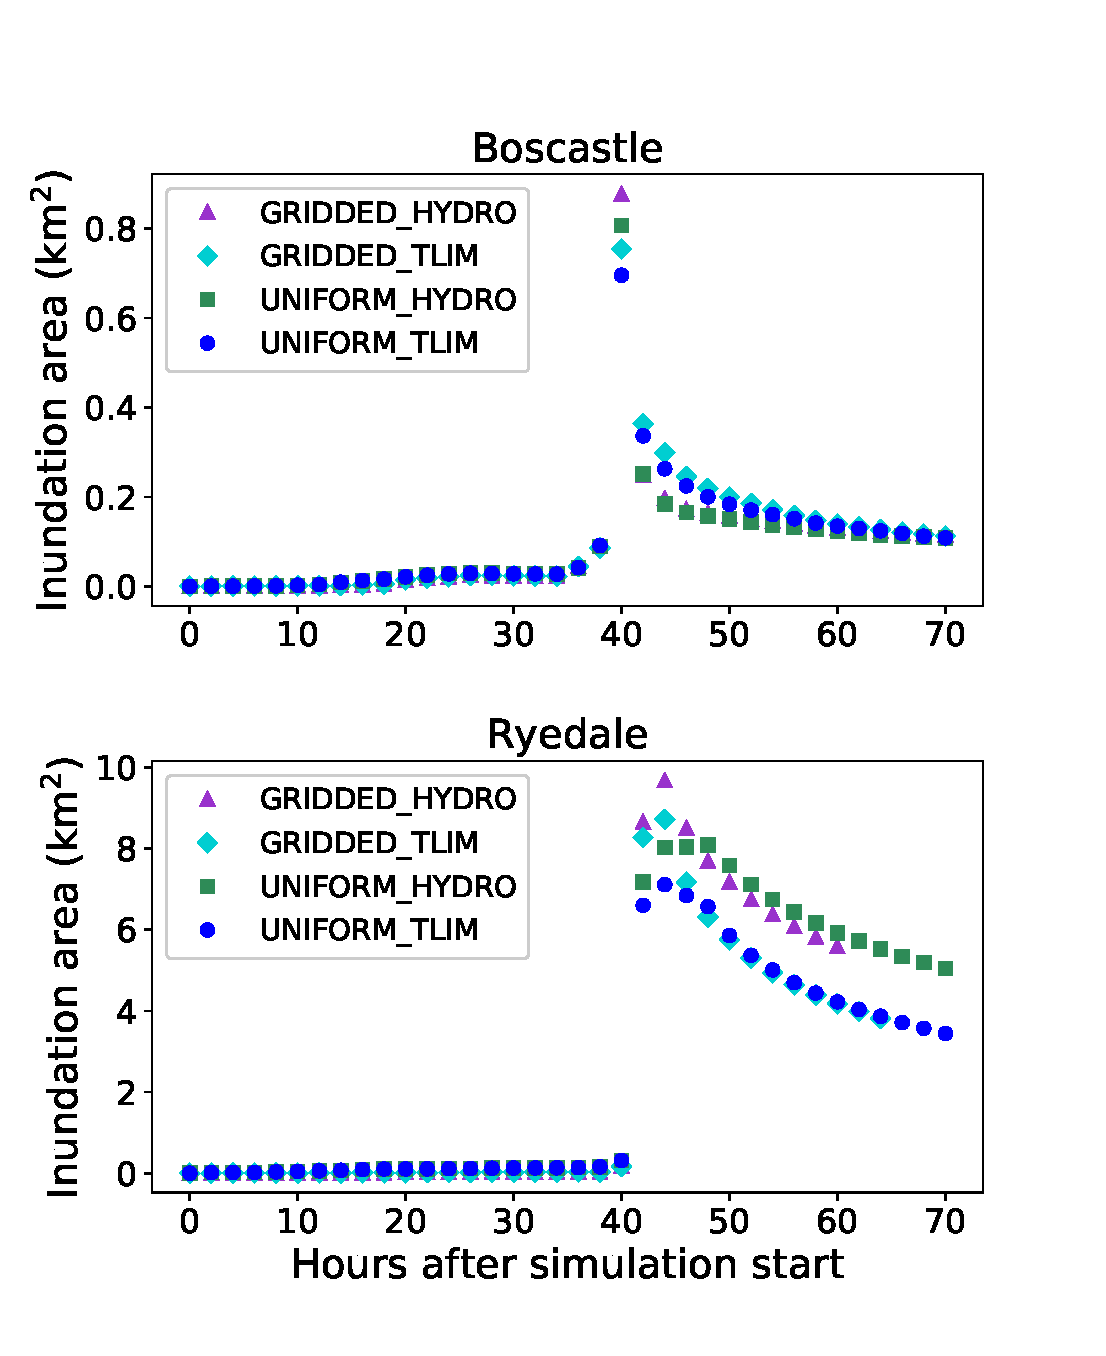
\includegraphics[width=12cm]{chp_flood_figs_scripts/inundation_area.eps}
\caption{Total inundation area (km$^2$) covered by floodwaters in the Boscastle (top) and Ryedale (bottom) catchments throughout the duration of the each storm. Inundation area is shown for each combination of flood-only, erosion-enabled, gridded rainfall input, and uniform rainfall input simulation. The erosion-enabled simulations use the transport-limited erosion law (\texttt{TLIM}). Detachment limited erosion cases were omitted for clarity.}
\label{fig_inundation_area_ensemble}
\end{figure}

\begin{figure}[!htbp]
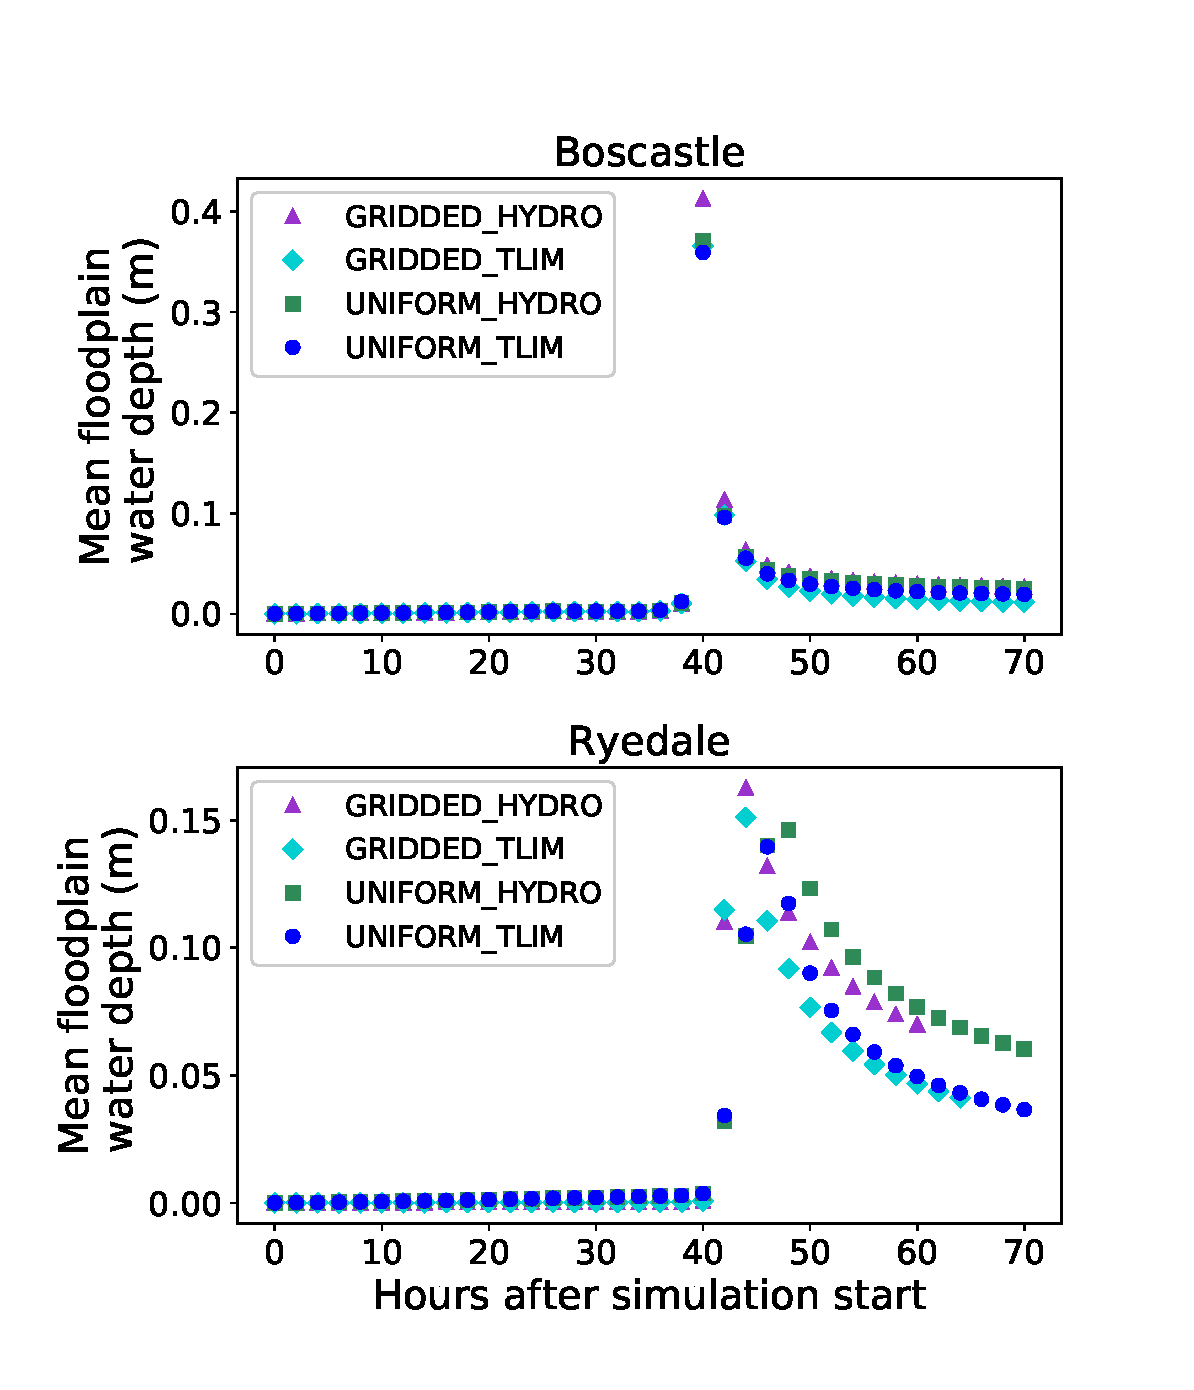
\includegraphics[width=12cm]{chp_flood_figs_scripts/floodplain_mean_depth.eps}
\caption{Mean floodplain water depth (metres) in the Boscastle (top) and Ryedale (bottom) catchments throughout the duration of the each storm. Floodplain is defined using the \citet{clubbinpress} floodplain delineation algorithm.) Water depth is shown for each combination of flood-only, erosion-enabled, gridded rainfall input, and uniform rainfall input simulation. The erosion-enabled simulations use the transport-limited erosion law (\texttt{TLIM}). Detachment limited erosion cases were omitted for clarity.}
\label{fig_floodplain_depth_ensemble}
\end{figure}

\begin{figure}[!htbp]
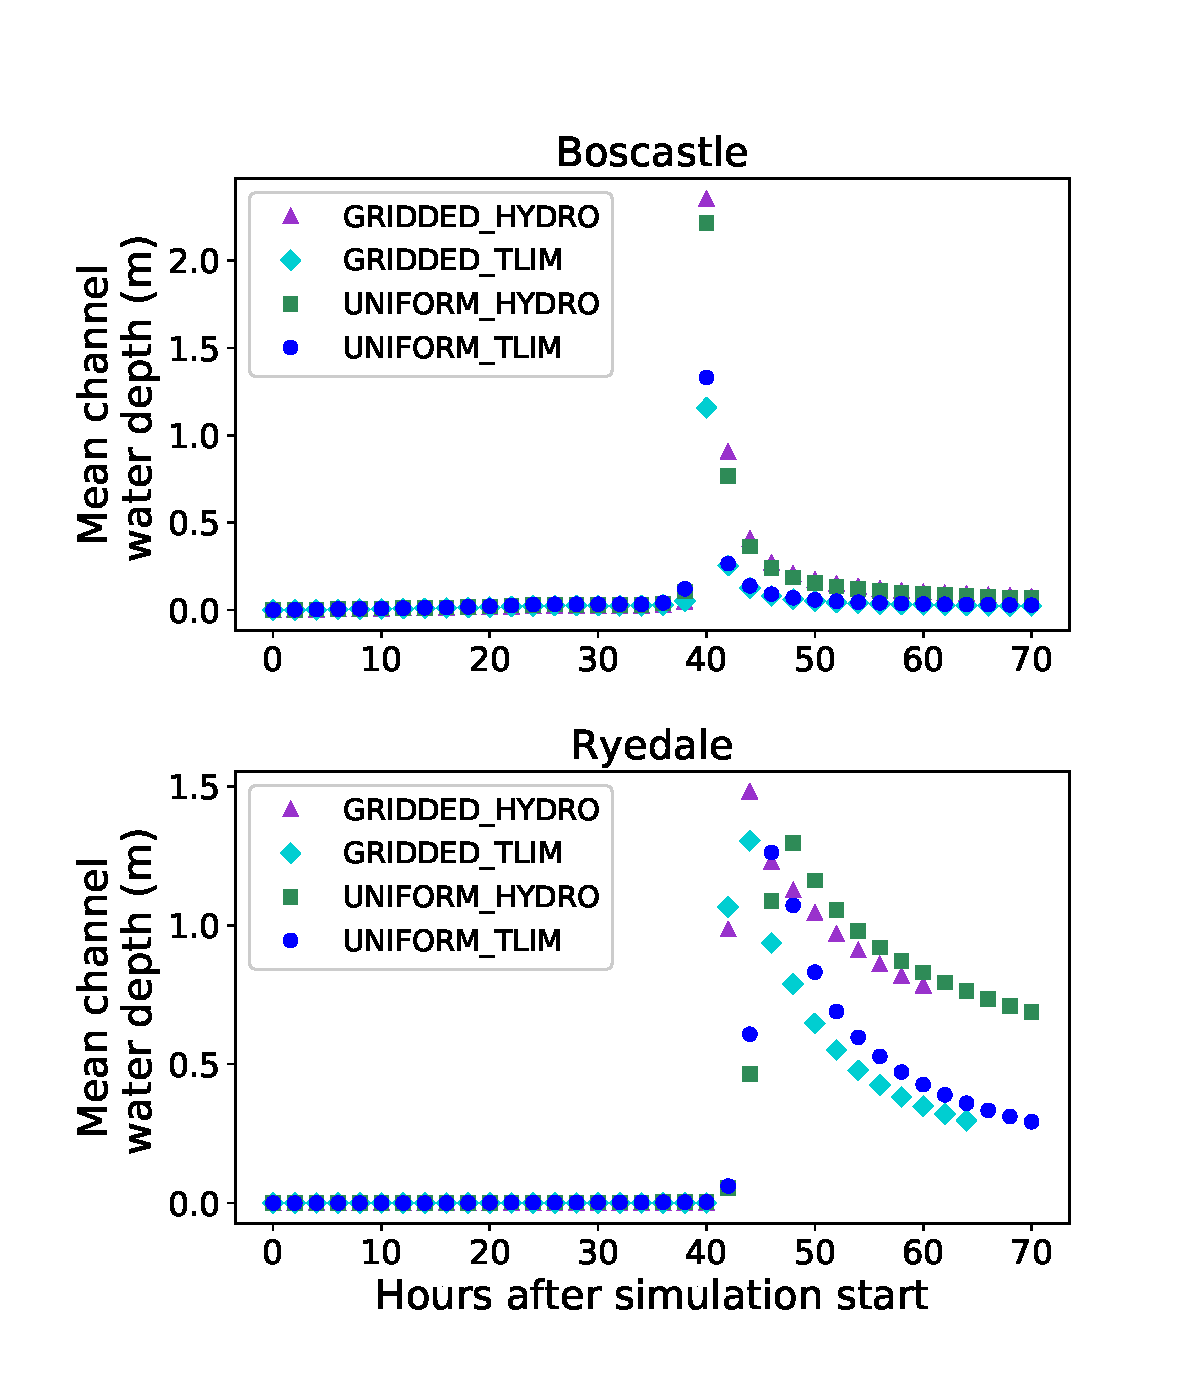
\includegraphics[width=12cm]{chp_flood_figs_scripts/channel_mean_depth.eps}
\caption{Main channel mean water depth (metres) in the Boscastle (top) and Ryedale (bottom) catchments throughout the duration of the each storm. The main channel is defined as the highest-order stream in each catchment \citep{strahler1957quantitative} and excludes all minor tributaries. Water depth is shown for each combination of flood-only, erosion-enabled, gridded rainfall input, and uniform rainfall input simulation. The erosion-enabled simulations use the transport-limited erosion law (\texttt{TLIM}). Detachment limited erosion cases were omitted for clarity.}
\label{fig_channel_depth_ensemble}
\end{figure}


\subsection{Spatial variation in flood inundation}
Thus far, the analysis of the model output has concerned catchment wide hydrological outputs and average water depths during flooding in the form of two-dimensional time series. The following section considers the spatial distribution of floodwaters across the catchments at the peak of each flood event. Comparisons between the spatial distribution of floodwaters under different model parameterisations are presented in Figures \ref{fig_boscastle_2dplan_flood_ensemble_town}, \ref{fig_boscastle_2dplan_flood_ensemble_confluence} (Boscastle), and Figures \ref{fig_ryedale_2dplan_flood_ensemble_floodplain}, \ref{fig_ryedale_2dplan_flood_ensemble_town}, \ref{fig_ryedale_2dplan_flood_ensemble_upstream} (Ryedale). An overview of the catchments and location of the main settlement in each is presented in Figure \ref{fig_boscastle_2dplan_inset_loc} and \ref{fig_ryedale_2dplan_location_insets}.

\subsubsection{Boscastle}
The Boscastle catchment simulations showed minimal variation in flood inundation extent. Simulations with gridded rainfall input did not result in substantially different predictions of floodwater inundation compared to those with uniform rainfall input. Both sets of simulations reflected the general extent of reported flood water extents \citep{wallingford2005flooding}. Simulations that allowed erosion to take place (\texttt{GRID\_TLIM} and \texttt{UNIFORM\_TLIM}) showed a slight difference in the variation of floodwater depths in the floodplain area, particularly in the vicinity of Boscastle village, where Figure \ref{fig_boscastle_2dplan_flood_ensemble_town} is centred on. In hydrological-only simulations, the deepest water depths were predicted to occur in the confines of the river channel, whereas in erosion-enabled simulations, there appeared to be a `smoothing' effect of water depths between the channel and the adjacent floodplain, suggesting that the channel geometry had altered during the flood event either by infilling from sediment from upstream or collapse of the adjacent river banks -- this effect is particularly evident in Figure \ref{fig_boscastle_2dplan_flood_ensemble_confluence}. Post-event reports of the Boscastle flood noted that the river channel in the Boscastle village area had indeed been inundated with debris during the storm, which had potentially contributed to the extent of the flooding within the village. The debris blockage of the  river channel as it flowed under the road bridge in the centre of the village was also noted as a potential contributory factor to the pattern of flood inundation during the storm. Overall, the results from the Boscastle simulations indicate that although the general differences in flood extent are minimal, there are small localised variations in the distribution of flood water depths at key locations, which can be attributed to the parameterisation of erosional processes in the simulations (Figure \ref{fig_boscastle_2dplan_flood_ensemble_town} and \ref{fig_boscastle_2dplan_flood_ensemble_confluence}).

\subsubsection{Ryedale}
The Ryedale simulations showed less variation in flood extents between the gridded rainfall and uniform rainfall inputs. The flood extents were only slightly greater in the gridded rainfall input simulations, despite the much higher peak discharges predicted in these simulations (Figure \ref{fig_ryedale_hydrograph_ensemble}). The main areas where flood extents were greater were in the floodplain area south of Helmsley (Figure \ref{fig_ryedale_2dplan_flood_ensemble_floodplain}) and in certain places around the settlement of Helmsley (Figure \ref{fig_ryedale_2dplan_flood_ensemble_town}).  The variation in water depths appeared to be less sensitive in comparison to the Boscastle simulations. In the lower reaches of the catchment (Figure \ref{fig_ryedale_2dplan_flood_ensemble_town}), there appeared to be little indication that flood extents or water depths were sensitive to the erosion parameterisation, in contrast to the Boscastle simulations.

%LOCATION MAP BOS
\begin{figure}[!htbp]
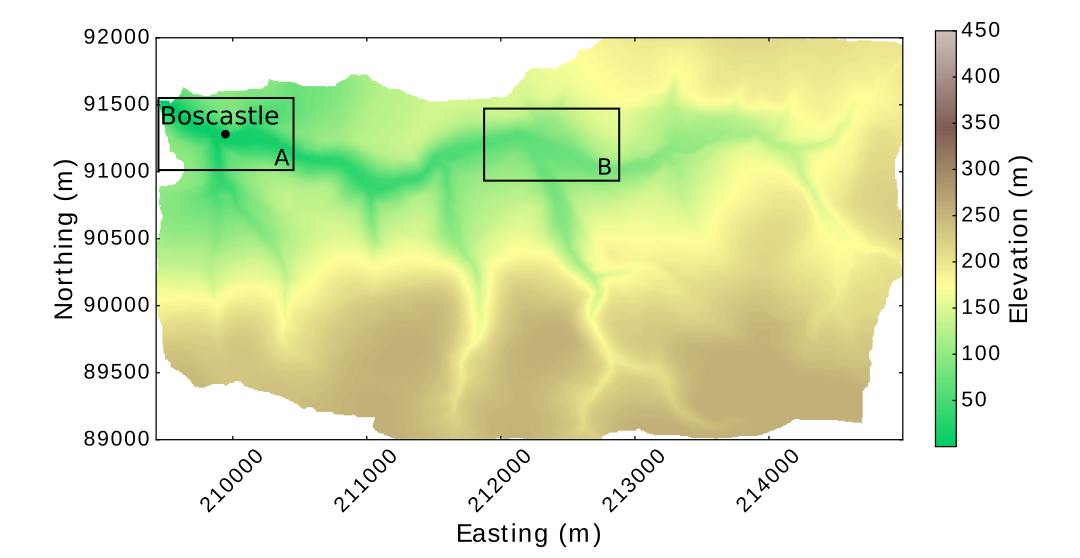
\includegraphics[width=14cm]{chp_flood_figs_scripts/fig_boscastle_catchment_insets.png}
\caption{Location map of the Boscastle catchment and Valency river valley, with the village of Boscastle shown. Location of the zoom-in images in Figures \ref{fig_boscastle_2dplan_flood_ensemble_town} (A) and \ref{fig_boscastle_2dplan_flood_ensemble_confluence} (B) shown in rectangular outlines.}
\label{fig_boscastle_2dplan_inset_loc}
\end{figure}

% Plan view flood maps BOSCASTLE
\begin{sidewaysfigure}[!htbp]
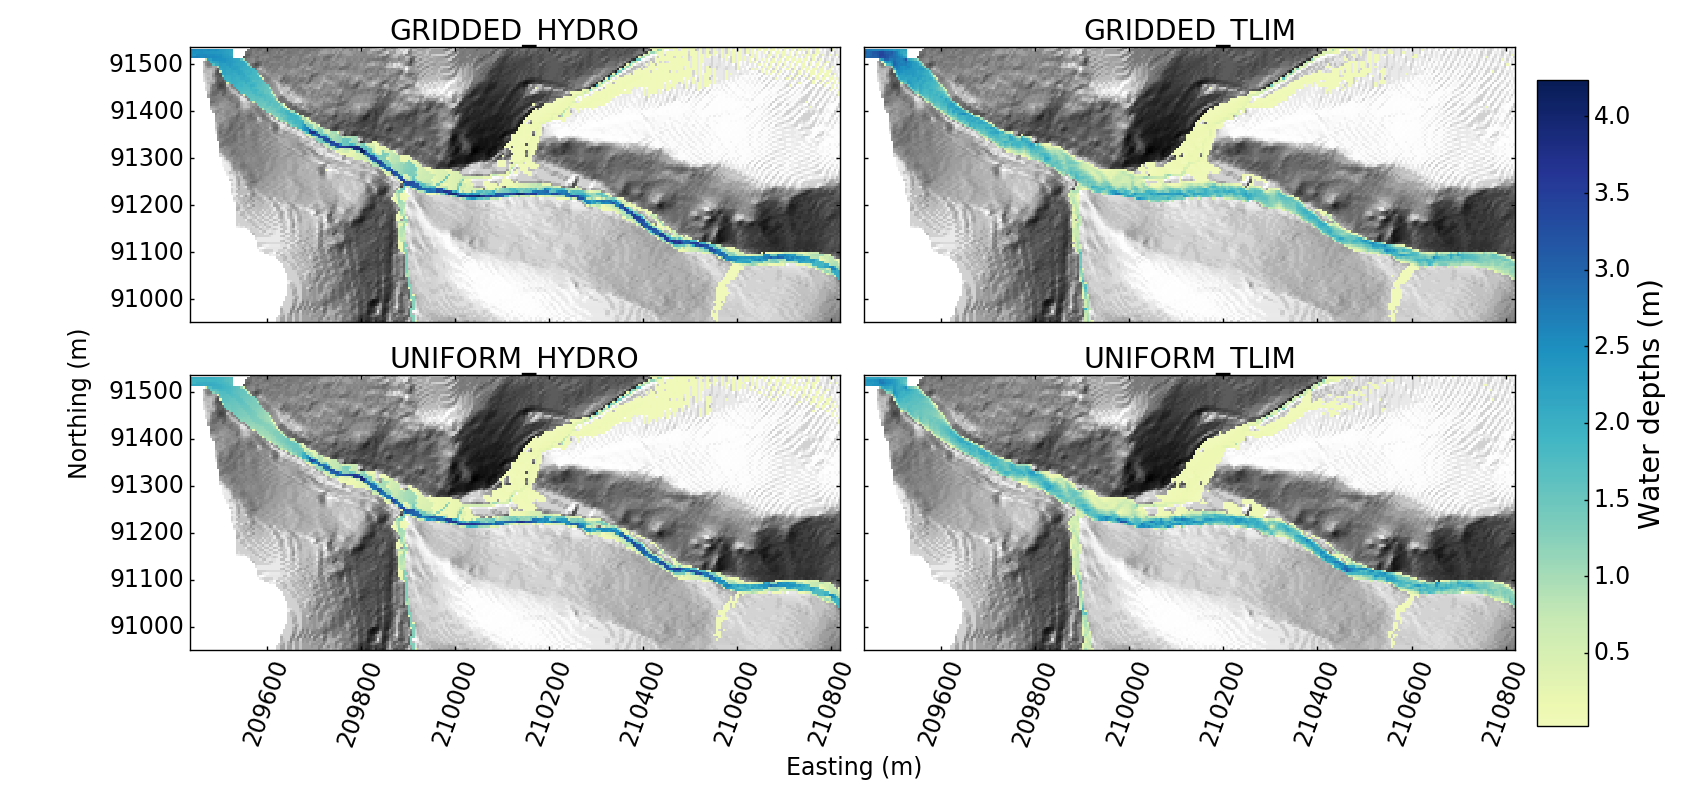
\includegraphics[width=24cm]{chp_flood_figs_scripts/fig_boscastle_flood_enseble_town.png}
\caption{Flood extents in the Boscastle catchment around the village area (location A on the overview map in Figure \ref{fig_boscastle_2dplan_inset_loc}) at the time of maximum river discharge for each simulation. }
\label{fig_boscastle_2dplan_flood_ensemble_town}
\end{sidewaysfigure}

\begin{sidewaysfigure}[!htbp]
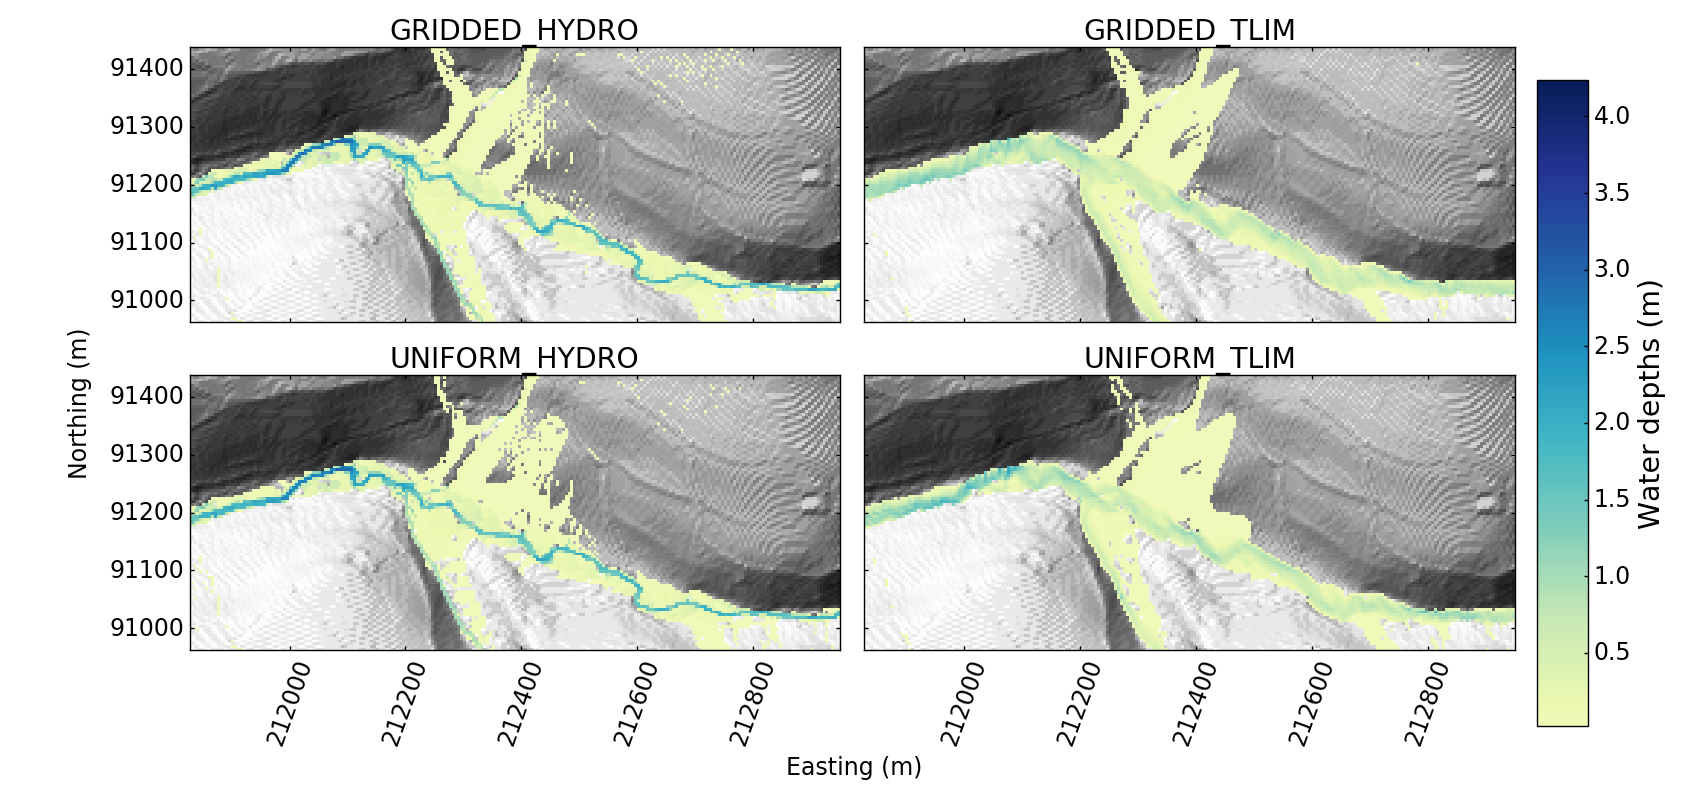
\includegraphics[width=24cm]{chp_flood_figs_scripts/fig_boscastle_flood_enseble_confluence.png}
\caption{Flood extents in the Boscastle catchment around the upstream confluence area (location B on the overview map in Figure \ref{fig_boscastle_2dplan_inset_loc}) at the time of maximum river discharge for each simulation.}
\label{fig_boscastle_2dplan_flood_ensemble_confluence}
\end{sidewaysfigure}

% Plan view flood  maps RYEDALE
\begin{figure}[!htbp]
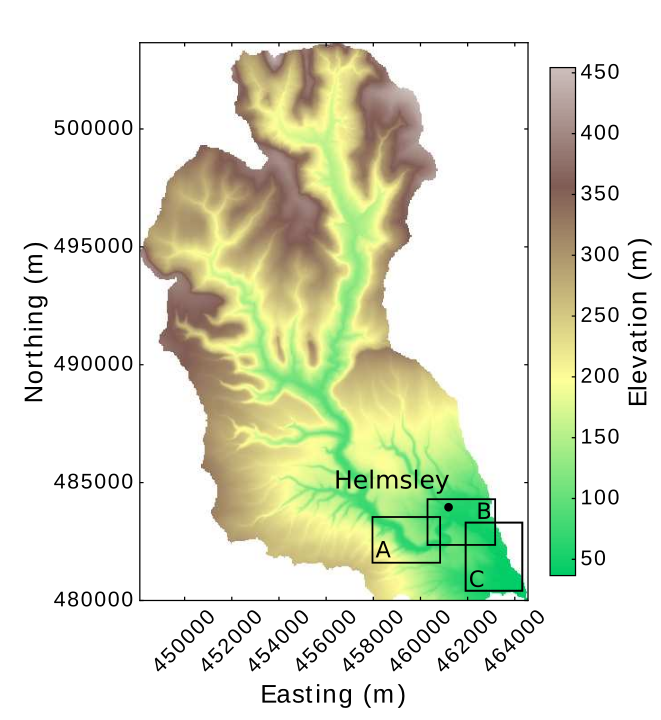
\includegraphics[width=12cm]{chp_flood_figs_scripts/fig_ryedale_catchment_location_insets.png}
\caption{Location map of the Ryedale catchment and Rye river valley, with the village of Helmsley shown. Location of the zoom-in images in Figures \ref{fig_ryedale_2dplan_flood_ensemble_floodplain} (A), \ref{fig_ryedale_2dplan_flood_ensemble_town} (B), and \ref{fig_ryedale_2dplan_flood_ensemble_upstream} (C) shown in rectangular outlines.}
\label{fig_ryedale_2dplan_location_insets}
\end{figure}

\begin{sidewaysfigure}[!htbp]
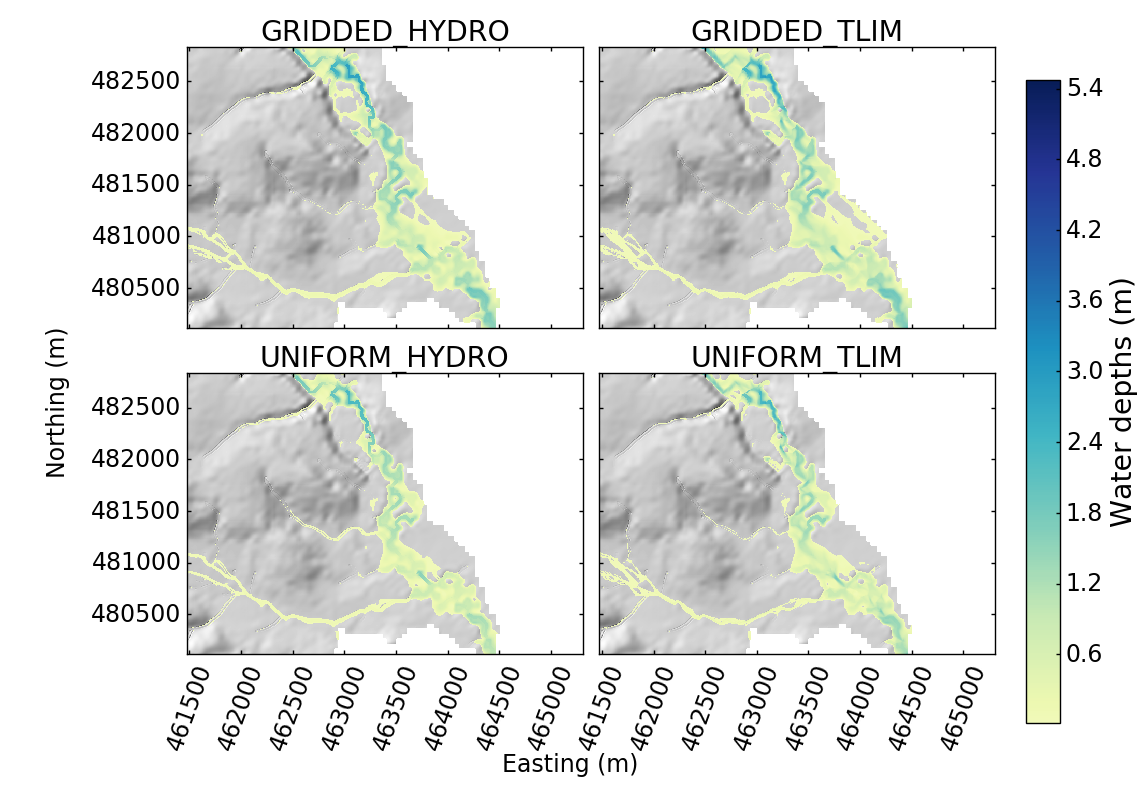
\includegraphics[width=20cm]{chp_flood_figs_scripts/fig_ryedale_flood_ensemble_floodplain.png}
\caption{Flood extents in the Ryedale catchment in the floodplain area south of Helmsley (location C on the overview map in Figure \ref{fig_ryedale_2dplan_location_insets}) at the time of maximum river discharge for each simulation.}
\label{fig_ryedale_2dplan_flood_ensemble_floodplain}
\end{sidewaysfigure}

\begin{sidewaysfigure}[!htbp]
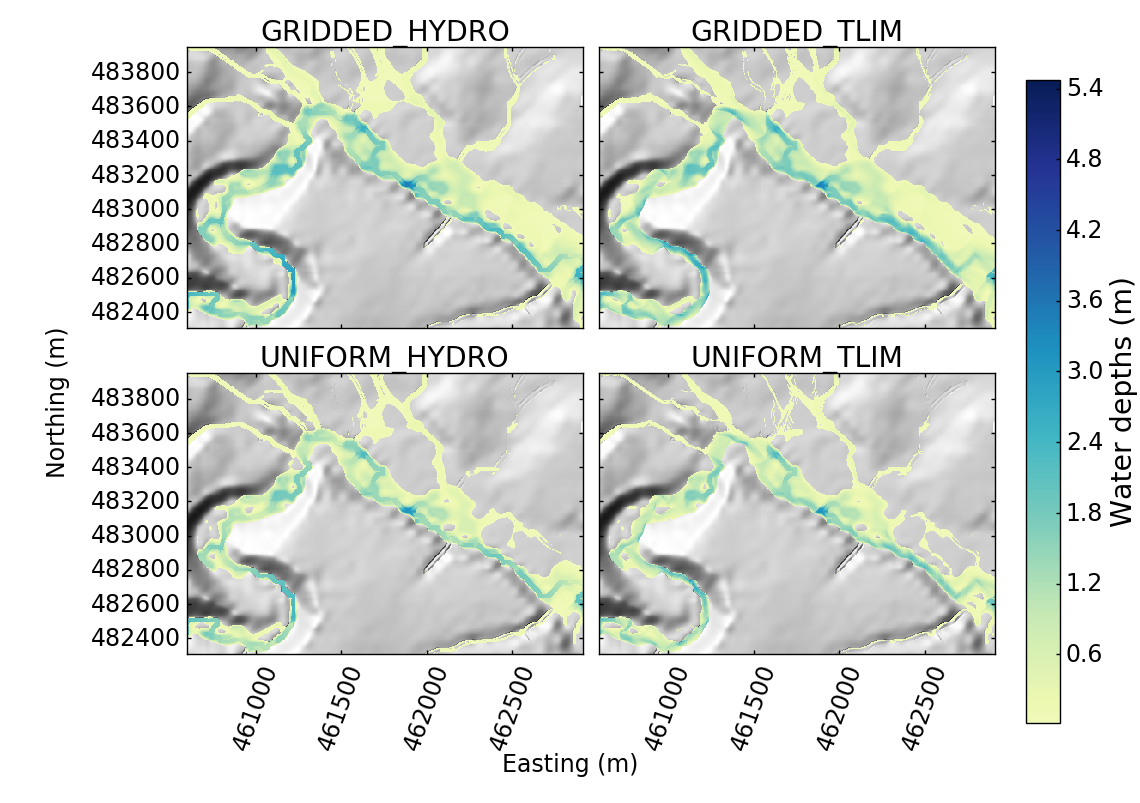
\includegraphics[width=20cm]{chp_flood_figs_scripts/fig_ryedale_flood_ensemble_helmsely.png}
\caption{Flood extents in the Ryedale catchment in the area surrounding Helmsley village (location B on the overview map in Figure \ref{fig_ryedale_2dplan_location_insets}) at the time of maximum river discharge for each simulation.}
\label{fig_ryedale_2dplan_flood_ensemble_town}
\end{sidewaysfigure}

\begin{sidewaysfigure}[!htbp]
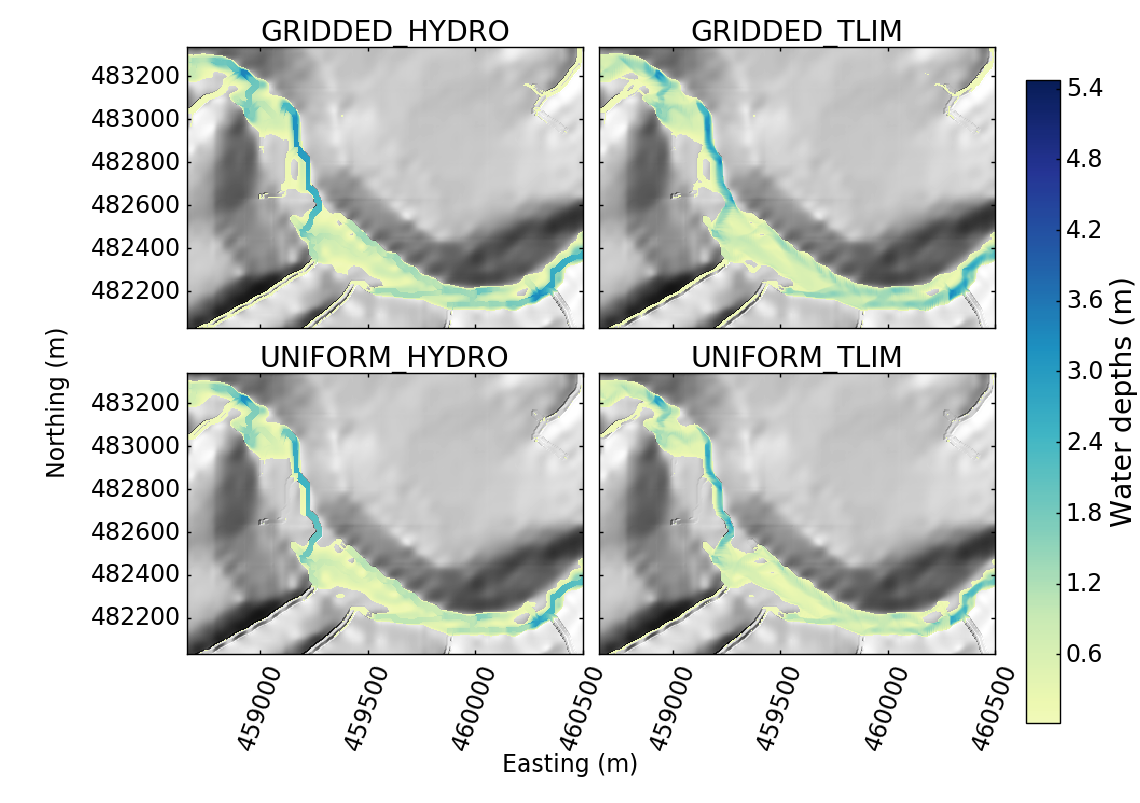
\includegraphics[width=20cm]{chp_flood_figs_scripts/fig_ryedale_flood_ensemble_upstream.png}
\caption{Flood extents in the Ryedale catchment in the gorge area west of Helmsley village (location A on the overview map in Figure \ref{fig_ryedale_2dplan_location_insets}) at the time of maximum river discharge for each simulation.}
\label{fig_ryedale_2dplan_flood_ensemble_upstream}
\end{sidewaysfigure}

\section{Discussion}

The aim of this chapter was to explore how modelled flood hydrology and flood inundation extents are sensitive to two external factors: the spatial resolution of precipitation inputs and the parameterisation of erosional processes. An ensemble simulation approach was taken using a cellular automaton landscape evolution and hydrological model to simulate two historic case studies of flash flooding events in the UK, varying the parameterisations of erosion and rainfall spatial resolution in each simulation. The results paint a complex picture of the competing controls of 1) spatial resolution of rainfall input and 2) erosional processes representation within the catchment.

\subsection{Rainfall spatial resolution}
In comparison to erosional parameterisation, the spatial resolution of rainfall input to the catchment exhibits a first-order control on its hydrological response during the flash flood event in both of the case studies presented here. Hydrographs from the Ryedale simulations were noticeably different in the prediction of the magnitude and timing of peak discharges, although in the smaller Boscastle catchment the differences in hydrological response were smaller, both in terms of the difference in timing of the peak flow and the peak water discharge rate. There are size differences between the two catchments studied -- the Ryedale catchment (270 km\(^2\)) is an order of magnitude larger in area than Boscastle (18 km\(^2\)) -- and such differences in catchment size have previously (although not conclusively) been argued to control the sensitivity of catchments to spatial variability in rainfall inputs \citep{krajewski1991monte,nicotina2008impact}. Although it has been argued that smaller catchments up to around 3500 km\(^2\) are largely insensitive to spatial variability in rainfall input due to a alack of heterogeneity in rainfall structures relative to the size of the catchment\citep{nicotina2008impact}, the results in this study suggest catchments around 250 km\(^2\) in size are sensitive to the spatial variability in rainfall inputs during intense rainfall events. For each simulation using gridded rainfall input, the cell width of the rainfall grid is 1 km. The relative amount of increase in rainfall detail between uniform and gridded simulations is potentially much greater in the larger Ryedale catchment than the Boscastle catchment. By using a 1 km gridded rainfall product as input data, the Ryedale simulation potentially captures 15 times more rainfall heterogeneity compared to the respective Boscastle simulation, by virtue of it simply being a much larger catchment with a greater number of rainfall input cells. 

The results from this study support the general consensus that there is some degree of sensitivity in catchment hydrology to rainfall spatial inputs, but in contrast to other studies, this sensitivity may be observed in much smaller catchments than previously thought. Furthermore, the flood inundation model used in this study appears to be more sensitive to spatial heterogeneity in rainfall inputs than it is to erosional parameterisation within the model, which may extend to hydrological modelling and flood forecasting in general. Further studies with different numerical models and different rainfall events would be needed to confirm this. 

The findings here potentially offer some explanation to other other studies that have shown over longer timescales, hydrological outputs from catchments simulated with spatially variable rainfall input data can see significant increases in mean annual discharge \citep{coulthard2016sensitivity}. If individual events can show notable differences in hydrological outputs, over time this will lead to larger differences in mean annual discharges. The general idea of catchment-size sensitivity to rainfall inputs is not challenged, but there is still a lack of consensus at what spatial scale this becomes an dominating factor. These findings suggest that catchments smaller than previously thought are also sensitive to rainfall spatial heterogeneity.

A further aim of this study was to investigate whether spatially detailed rainfall data leads to more accurate hydrological predictions, not merely \textit{different} predictions. Where available, measurements of the timing, magnitude, and spatial distribution of flood inundation were compared with the predictions made by the numerical model. Both the Ryedale and Boscastle events were extensively studied and surveyed in their aftermath and comparisons with previous modelling studies of each event were made where these were available. With respect to the aim of improving the accuracy of flood inundation predictions with high-resolution rainfall data, the results were mixed. For the Boscastle case study, there was better agreement with the peak discharges published in the \citet{wallingford2005flooding} report when using the gridded rainfall input to drive the numerical model, though a limitation of this comparison is that the hydrographs published in the HR Wallingford report were themselves based on estimates from eyewitness observations, reconstructions from water-level marks, and one-dimensional hydraulic modelling. Nonetheless, the better agreement with other published findings is encouraging for the case of using high-resolution rainfall data in hydrological models.

In the Ryedale case study, using gridded rainfall input actually produced a less accurate prediction of the peak discharge during the flood, though the only comparison available was made with a single gauge station at the catchment outlet -- gauging station data can be unreliable during extreme flows and this may partly explain the discrepancy. In this case, the uniform rainfall data actually gave a better hydrological prediction in terms of matching the timing and rate of peak discharge during the flood. 

% More on the m value, equifinality, Welsh study 2009.
\subsection{Choice of \(m\) parameter value}
The sensitivity analysis of the model \(m\) parameter was initially done using one type of rainfall input (spatially uniform) for the Ryedale catchment, and the value of \(m\) that most closely matched published hydrographs (\(m = 0.005\)) was used for all of the simulations in Table \ref{table_ensemble_experiments}. Subsequent analysis showed that a separate sensitivity analyses using the gridded rainfall input revealed a different `best-fit' value of \(m=0.0075\) when using the gridded rainfall input (Figure \ref{fig_topmodel_m_ryedale_gridded}), leading to better hydrological predictions from the gridded rainfall input simulations. This raises the issue that the model can be configured with different parameters and arrive at the same or similar predictions -- a concept referred to as equifinality and one which is often encountered in the hydrological modelling community \citep{beven1993prophecy,beven2001equifinality,ebel2006physics} -- which somewhat limits the conclusions that can be drawn from the experiments comparing uniform rainfall inputs with gridded rainfall input. In this particular case, both choices of \(m\) value are within reasonable ranges for the types of environment simulated \citep{beven1984testing}, but depending on the choice of \(m\) value, the case for using spatially variable rainfall inputs can be either strengthed or weakened. Does one chose to calibrate the model based on the type of rainfall spatial input as well, and if so, should it be calibrated further based on the type of erosional parametrisation enabled in the model? The size of the parameter space in the HAIL-CAESAR model is large, and a systematic exploration of every single combination of parameters would be time consuming if it were required for every case study to be simulated. Answering these questions of model calibration is beyond the scope of this study, but a recommendation can be made for future studies using the TOPMODEL-based runoff generation in models to assess the sensitivity to the \(m\) parameter as hydrological outputs may be highly sensitive to its value.

% Discussion on erosional parameterisation.
\subsection{Erosional parameterisation}
The results of the numerical modelling simulations suggested that choice of erosional parameterisation exerts a secondary control on the hydrological response of a catchment when compared to the effects of the choice in rainfall resolution input. Consistently across simulations, the enabling of a transport-limited (\texttt{TLIM}) erosional parameterisation in the HAIL-CAESAR model resulted in higher predicted peak discharges, evident in both the gridded rainfall and uniform rainfall sets of simulations. Again, the size of the catchment appears to be a factor in determining the degree of sensitivity, with the differences in hydrological output greater in the larger Ryedale catchment when using erosion-enabled simulations. The differences in discharge, however, are relatively smaller in both cases and any change in discharge from varying the choice of erosion law is surpassed by using a gridded rainfall input source over a spatially uniform one.

The same limited sensitivity to erosional parameterisation is noted by \citep{wong2015sensitivity}, using a similar hydraulic model to investigate flood inundation sensitivity to channel morphological change during flood events. The hydraulic model used in the \citet{wong2015sensitivity} study is based on the same two-dimensional flood inundation model used in HAIL-CAESAR, coupled with a simple erosional model that allows the channel bed elevation to be eroded (but no sediment deposited) during the course of a flood. \citet{wong2015sensitivity} note that differences in hydrological response are minimal during erosion-enabled simulations, athough there is a small increase of up to 5\% in the simulated mean depth of floodwaters throughout the event they simulate. By contrast, the results presented here show that floodwater depths on average are lower in erosion-enabled simulations. The erosion-enabled simulations presented in this chapter address a limitation in the \citet{wong2015sensitivity} study in that they permit the redistribution of sediments within a catchment through depositional as well as erosional processes.  In theory, such a model could capture channel blockage from sediment build up or infill during a flood, although this behaviour is not immediately apparent from the simulations carried out for these case studies. However, considering the sets of gridded-and uniform-rainfall input simulations separately, the predicted mean water depths in the main channel of each catchment (Figure \ref{fig_channel_depth_ensemble}) are lower in the erosion-enabled simulations indicating that sediment infill of the channels has taken place and reduced water depths in the channels. In the Boscastle simulations, the mean water depths are as much as 1 m lower in the transport-limited erosion-enabled simulations than the corresponding hydrology-only simulations where the morphology of the channel bed and floodplain are effectively fixed. Average floodplain water depths are also lower in the erosion-enabled Boscastle simulations (Figure \ref{fig_floodplain_depth_ensemble}). An alternative explanation for the lower water depths seen in the erosion-enabled simulations is that the coarse model output time step (two-hourly) simply did not capture the exact timing of peak flood water extent, and so the recorded depths for the erosion-enabled simulations are near to, but not quite, at the peak of flood inundation.

In models that permit the channel to be lowered through erosional processes, but no sediment deposition to take place, the channel and floodplain capacity to store or transport water can only be increased during the flood \citep[e.g.][]{wong2015sensitivity}. The effect of this could either be to increase the rate of water transport downstream through the channels to the floodplains, or to increase the channel capacity to store water during the course of the flood. In \citet{wong2015sensitivity} the case seems to have been that water depths have increased on the floodplain when erosion was enabled in their model. In models that permit both channel erosion and sediment deposition,  the possibility arises that channel capacity is reduced during the flood through the deposition of sediments in the channel. However, detailed observational evidence recorded after the Boscastle event tends not to support this hypothesis as the amount of floodplain deposited sediments was on the order of centimetres, and most sections of the channel underwent net incision rather than deposition. In any case, a detailed analysis of the change in channel carrying capacity was beyond the scope of this study, but a change in channel capacity is a potential explanation for some of the differences seen between  \citet{wong2015sensitivity} and the results of this analysis. A further explanation for the general lack of hydrological sensitivity to morphological changes to the channel and floodplain during large floods is that the channel and floodplain act as a single channel unit \citep{bates2005numerical}, and so localised changes to one hydromorphic feature are compensated for by the other, in effect dampening any potential hydrological sensitivity to erosional processes.


%%%%%%%%%%%%%%%%%%%%%
\section{Conclusions}  %% \conclusions[modified heading if necessary]
%%%%%%%%%%%%%%%%%%%%%
Considering the competing factors of spatial variation in rainfall inputs and erosional parameterisation in hydrological models, two main conclusions can be drawn from this investigation:

\paragraph{Rainfall resolution}
In distributed models of catchment hydrology, rainfall input data that is spatially variable is likely to lead to greater hydrological outputs during severe rainfall events. The probable cause of increased water outputs is that localised peaks in rainfall rate are captured by the use of high-resolution rainfall data, such as meteorological radar, that would otherwise be smoothed-out by spatially uniform rainfall inputs or coarser resolution rainfall data. This conclusion, however, assumes that rainfall structures themselves are spatially heterogeneous relative to the size of the catchment being modelled. Catchment size itself may be a controlling factor determining how sensitive the hydrological response is to spatially detailed rainfall input data, but another possible explanation is that it is the ratio of rainfall detail captured in input data, relative to the size of the catchment. A further systematic study investigating hydrological sensitivity to a range of rainfall structures of varying structural complexity would be needed to assess this hypothesis. 

Higher-resolution rainfall input data has the potential to improve the accuracy of hydrological predictions, but it is not conclusive that this is always the case based on the results of this study. For high-resolution rainfall data to be of use to hydrological modellers, the other parameters within the model must be well constrained, either through field study (where parameters can be constrained through field measurement), detailed exploration of parameter sensitivity and calibration of the model, or a combination of both. 

\paragraph{Erosional parameterisation}
Hydrological simulations show some sensitivity to erosional parameterisation. The amount of change in hydrological outputs and spatial distribution of flood waters is small relative to the sensitivity to rainfall spatial heterogeneity. The conclusions in this respect are similar to that of \citet{wong2015sensitivity} in that getting an accurate representation of erosional process in hydrological models is likely to be of secondary importance compared to obtaining accurate inputs of rainfall intensity and distribution. Errors in the radar-derived rainfall rate and in the radar-derived spatial distribution of rainfall are more likely to have a larger impact on model performance compared to the nuances in flood dynamics predicted by erosion-enabled simulations. An often reported consequence of large flood events is that bridged channels and culverts can become blocked  with mobilised debris (other than sediment), leading to localised changes in flood dynamics. A limitation of the HAIL-CAESAR model, and others like it, is that they cannot account for closed-channel flow and blockages from debris, but future model enhancements may enable this kind of localised change in flood hydraulics to be investigated further.

\subsubsection{Summary}
Hydrological modelling shows measurable sensitivity to the spatial variation in rainfall inputs using gridded rainfall data derived from meteorological radar. Sensitivity is more pronounced in larger catchments, though it is also noticeable in smaller catchments during extreme flood events, contrary to previously published studies. Whether or not high-resolution  rainfall data can improve hydrological model performance depends on the constraint of other model parameters, notably the \(m\) parameter, that can lead to large amounts of uncertainty in the hydrological response of a catchment to intense rainfall. Erosional parameterisation within a hydrological model -- the ability to represent changes in channel and floodplain morphology during a flash flood event -- appears to be of only secondary importance in determining the hydrological response based on the studies carried out in this investigation. Nonetheless, both erosional parameterisation and spatial distribution of rainfall remain important factors to be considered in future models of flood inundation and catchment hydrology.




%\printbibliography
%\end{refsection}
